% =====================================================================
%  WORKING COPY of the thesis (Smart Supply Chain Management System).
%  - Same preamble/formatting as the original main.tex (UNCHANGED template).
%  - Body content lives in NoiDung/*.tex  ->  YOU WRITE THERE.
%  - Build:  latexmk -pdf -outdir=build main_datn.tex
%  The original main.tex + Chapter/* are kept untouched as a reference.
% =====================================================================
\documentclass[a4paper,13pt,3p,twoside]{report}
\usepackage{scrextend}
\changefontsizes{13pt}
\usepackage[utf8]{vietnam}
\usepackage[top=2cm, bottom=2cm, left=3.5cm, right=2.5cm]{geometry}

\usepackage{graphicx}
\usepackage{fancybox}
\usepackage{indentfirst}
\usepackage{amsthm}
\usepackage{latexsym}
\usepackage{amsmath}
\usepackage{amssymb}
\usepackage{amsbsy}
\usepackage{times}
\usepackage{array}
\usepackage{enumitem}
\usepackage{subfiles}
\usepackage{titlesec}
\usepackage{titletoc}
\usepackage{chngcntr}
\usepackage{pdflscape}
\usepackage{afterpage}
\usepackage[ruled,vlined]{algorithm2e}
\usepackage{capt-of}
\usepackage{multirow}
\usepackage{fancyhdr}
\usepackage{appendix}
\usepackage{outlines}
\usepackage[font=small,labelfont=bf]{caption}

\usepackage{listings}
\usepackage{float}
\usepackage{subcaption}
\usepackage{xurl}
\usepackage{longtable}
\usepackage{booktabs}

\usepackage[nonumberlist, nopostdot, nogroupskip, acronym]{glossaries}
\usepackage{glossary-superragged}
\setglossarystyle{superraggedheaderborder}
\usepackage{setspace}
\usepackage{parskip}

\usepackage{tocbasic}
\usepackage{blindtext}

% ===================================================
\renewcommand{\bibname}{reference}
\usepackage[backend=bibtex,style=ieee]{biblatex}

\renewcommand\appendixname{APPENDIX}
\renewcommand\appendixpagename{APPENDIX}
\renewcommand\appendixtocname{APPENDIX}

\renewcommand{\figurename}{Figure}
\renewcommand{\tablename}{Table}
\renewcommand{\chaptername}{CHAPTER}

\addbibresource{reference.bib}

% ============================================================
% Cấu hình chèn và định dạng mã nguồn (listings)
% Dùng cho đồ án: Java / Spring Boot, SQL, JSON...
% File này được nạp bởi % ============================================================
% Cấu hình chèn và định dạng mã nguồn (listings)
% Dùng cho đồ án: Java / Spring Boot, SQL, JSON...
% File này được nạp bởi % ============================================================
% Cấu hình chèn và định dạng mã nguồn (listings)
% Dùng cho đồ án: Java / Spring Boot, SQL, JSON...
% File này được nạp bởi \include{lstlisting} trong main.tex
% ============================================================
\usepackage{listings}
\usepackage{xcolor}

% --- Bảng màu ---
\definecolor{codegreen}{rgb}{0.0,0.5,0.0}    % comment
\definecolor{codeblue}{rgb}{0.0,0.0,0.7}     % keyword
\definecolor{codepurple}{rgb}{0.58,0.0,0.82} % string
\definecolor{codegray}{rgb}{0.5,0.5,0.5}     % số dòng
\definecolor{backcolour}{rgb}{0.97,0.97,0.95}% nền

% --- Style chung ---
\lstdefinestyle{datnstyle}{
    backgroundcolor=\color{backcolour},
    commentstyle=\color{codegreen}\itshape,
    keywordstyle=\color{codeblue}\bfseries,
    numberstyle=\tiny\color{codegray},
    stringstyle=\color{codepurple},
    basicstyle=\ttfamily\footnotesize,
    breakatwhitespace=false,
    breaklines=true,
    captionpos=b,
    keepspaces=true,
    numbers=left,
    numbersep=8pt,
    showspaces=false,
    showstringspaces=false,
    showtabs=false,
    tabsize=2,
    frame=single,
    rulecolor=\color{codegray},
    xleftmargin=12pt,
    framexleftmargin=12pt,
    upquote=true,
    literate=
        {á}{{\'a}}1 {à}{{\`a}}1 {ả}{{\h{a}}}1 {ã}{{\~a}}1 {ạ}{{\d{a}}}1
        {â}{{\^a}}1 {ấ}{{\'{\^a}}}1 {ầ}{{\`{\^a}}}1 {ậ}{{\d{\^a}}}1
        {ă}{{\u{a}}}1 {đ}{{\dj}}1 {Đ}{{\DJ}}1
        {é}{{\'e}}1 {è}{{\`e}}1 {ê}{{\^e}}1 {ế}{{\'{\^e}}}1 {ệ}{{\d{\^e}}}1
        {í}{{\'i}}1 {ì}{{\`i}}1 {ị}{{\d{i}}}1
        {ó}{{\'o}}1 {ò}{{\`o}}1 {ô}{{\^o}}1 {ố}{{\'{\^o}}}1 {ộ}{{\d{\^o}}}1
        {ơ}{{\horn{o}}}1 {ớ}{{\'{\horn{o}}}}1 {ợ}{{\d{\horn{o}}}}1
        {ú}{{\'u}}1 {ù}{{\`u}}1 {ư}{{\horn{u}}}1 {ứ}{{\'{\horn{u}}}}1 {ự}{{\d{\horn{u}}}}1
        {ý}{{\'y}}1 {ỳ}{{\`y}}1
}

% Đặt style mặc định
\lstset{style=datnstyle}

% --- Định nghĩa thêm ngôn ngữ JSON (listings không có sẵn) ---
\lstdefinelanguage{json}{
    basicstyle=\ttfamily\footnotesize,
    stringstyle=\color{codepurple},
    showstringspaces=false,
    breaklines=true,
    frame=single,
    literate=
        *{:}{{{\color{codeblue}{:}}}}1
        {,}{{{\color{codeblue}{,}}}}1
        {\{}{{{\color{codeblue}{\{}}}}1
        {\}}{{{\color{codeblue}{\}}}}}1
        {[}{{{\color{codeblue}{[}}}}1
        {]}{{{\color{codeblue}{]}}}}1,
}

% ============================================================
% CÁCH DÙNG (ví dụ):
%
%   \begin{lstlisting}[language=Java, caption={Service xử lý đơn hàng}, label={lst:order}]
%   @Service
%   public class DeliveryOrderService { ... }
%   \end{lstlisting}
%
% Hoặc chèn từ file:
%   \lstinputlisting[language=SQL, caption={Schema kho}]{Figure/schema.sql}
% ============================================================
 trong main.tex
% ============================================================
\usepackage{listings}
\usepackage{xcolor}

% --- Bảng màu ---
\definecolor{codegreen}{rgb}{0.0,0.5,0.0}    % comment
\definecolor{codeblue}{rgb}{0.0,0.0,0.7}     % keyword
\definecolor{codepurple}{rgb}{0.58,0.0,0.82} % string
\definecolor{codegray}{rgb}{0.5,0.5,0.5}     % số dòng
\definecolor{backcolour}{rgb}{0.97,0.97,0.95}% nền

% --- Style chung ---
\lstdefinestyle{datnstyle}{
    backgroundcolor=\color{backcolour},
    commentstyle=\color{codegreen}\itshape,
    keywordstyle=\color{codeblue}\bfseries,
    numberstyle=\tiny\color{codegray},
    stringstyle=\color{codepurple},
    basicstyle=\ttfamily\footnotesize,
    breakatwhitespace=false,
    breaklines=true,
    captionpos=b,
    keepspaces=true,
    numbers=left,
    numbersep=8pt,
    showspaces=false,
    showstringspaces=false,
    showtabs=false,
    tabsize=2,
    frame=single,
    rulecolor=\color{codegray},
    xleftmargin=12pt,
    framexleftmargin=12pt,
    upquote=true,
    literate=
        {á}{{\'a}}1 {à}{{\`a}}1 {ả}{{\h{a}}}1 {ã}{{\~a}}1 {ạ}{{\d{a}}}1
        {â}{{\^a}}1 {ấ}{{\'{\^a}}}1 {ầ}{{\`{\^a}}}1 {ậ}{{\d{\^a}}}1
        {ă}{{\u{a}}}1 {đ}{{\dj}}1 {Đ}{{\DJ}}1
        {é}{{\'e}}1 {è}{{\`e}}1 {ê}{{\^e}}1 {ế}{{\'{\^e}}}1 {ệ}{{\d{\^e}}}1
        {í}{{\'i}}1 {ì}{{\`i}}1 {ị}{{\d{i}}}1
        {ó}{{\'o}}1 {ò}{{\`o}}1 {ô}{{\^o}}1 {ố}{{\'{\^o}}}1 {ộ}{{\d{\^o}}}1
        {ơ}{{\horn{o}}}1 {ớ}{{\'{\horn{o}}}}1 {ợ}{{\d{\horn{o}}}}1
        {ú}{{\'u}}1 {ù}{{\`u}}1 {ư}{{\horn{u}}}1 {ứ}{{\'{\horn{u}}}}1 {ự}{{\d{\horn{u}}}}1
        {ý}{{\'y}}1 {ỳ}{{\`y}}1
}

% Đặt style mặc định
\lstset{style=datnstyle}

% --- Định nghĩa thêm ngôn ngữ JSON (listings không có sẵn) ---
\lstdefinelanguage{json}{
    basicstyle=\ttfamily\footnotesize,
    stringstyle=\color{codepurple},
    showstringspaces=false,
    breaklines=true,
    frame=single,
    literate=
        *{:}{{{\color{codeblue}{:}}}}1
        {,}{{{\color{codeblue}{,}}}}1
        {\{}{{{\color{codeblue}{\{}}}}1
        {\}}{{{\color{codeblue}{\}}}}}1
        {[}{{{\color{codeblue}{[}}}}1
        {]}{{{\color{codeblue}{]}}}}1,
}

% ============================================================
% CÁCH DÙNG (ví dụ):
%
%   \begin{lstlisting}[language=Java, caption={Service xử lý đơn hàng}, label={lst:order}]
%   @Service
%   public class DeliveryOrderService { ... }
%   \end{lstlisting}
%
% Hoặc chèn từ file:
%   \lstinputlisting[language=SQL, caption={Schema kho}]{Figure/schema.sql}
% ============================================================
 trong main.tex
% ============================================================
\usepackage{listings}
\usepackage{xcolor}

% --- Bảng màu ---
\definecolor{codegreen}{rgb}{0.0,0.5,0.0}    % comment
\definecolor{codeblue}{rgb}{0.0,0.0,0.7}     % keyword
\definecolor{codepurple}{rgb}{0.58,0.0,0.82} % string
\definecolor{codegray}{rgb}{0.5,0.5,0.5}     % số dòng
\definecolor{backcolour}{rgb}{0.97,0.97,0.95}% nền

% --- Style chung ---
\lstdefinestyle{datnstyle}{
    backgroundcolor=\color{backcolour},
    commentstyle=\color{codegreen}\itshape,
    keywordstyle=\color{codeblue}\bfseries,
    numberstyle=\tiny\color{codegray},
    stringstyle=\color{codepurple},
    basicstyle=\ttfamily\footnotesize,
    breakatwhitespace=false,
    breaklines=true,
    captionpos=b,
    keepspaces=true,
    numbers=left,
    numbersep=8pt,
    showspaces=false,
    showstringspaces=false,
    showtabs=false,
    tabsize=2,
    frame=single,
    rulecolor=\color{codegray},
    xleftmargin=12pt,
    framexleftmargin=12pt,
    upquote=true,
    literate=
        {á}{{\'a}}1 {à}{{\`a}}1 {ả}{{\h{a}}}1 {ã}{{\~a}}1 {ạ}{{\d{a}}}1
        {â}{{\^a}}1 {ấ}{{\'{\^a}}}1 {ầ}{{\`{\^a}}}1 {ậ}{{\d{\^a}}}1
        {ă}{{\u{a}}}1 {đ}{{\dj}}1 {Đ}{{\DJ}}1
        {é}{{\'e}}1 {è}{{\`e}}1 {ê}{{\^e}}1 {ế}{{\'{\^e}}}1 {ệ}{{\d{\^e}}}1
        {í}{{\'i}}1 {ì}{{\`i}}1 {ị}{{\d{i}}}1
        {ó}{{\'o}}1 {ò}{{\`o}}1 {ô}{{\^o}}1 {ố}{{\'{\^o}}}1 {ộ}{{\d{\^o}}}1
        {ơ}{{\horn{o}}}1 {ớ}{{\'{\horn{o}}}}1 {ợ}{{\d{\horn{o}}}}1
        {ú}{{\'u}}1 {ù}{{\`u}}1 {ư}{{\horn{u}}}1 {ứ}{{\'{\horn{u}}}}1 {ự}{{\d{\horn{u}}}}1
        {ý}{{\'y}}1 {ỳ}{{\`y}}1
}

% Đặt style mặc định
\lstset{style=datnstyle}

% --- Định nghĩa thêm ngôn ngữ JSON (listings không có sẵn) ---
\lstdefinelanguage{json}{
    basicstyle=\ttfamily\footnotesize,
    stringstyle=\color{codepurple},
    showstringspaces=false,
    breaklines=true,
    frame=single,
    literate=
        *{:}{{{\color{codeblue}{:}}}}1
        {,}{{{\color{codeblue}{,}}}}1
        {\{}{{{\color{codeblue}{\{}}}}1
        {\}}{{{\color{codeblue}{\}}}}}1
        {[}{{{\color{codeblue}{[}}}}1
        {]}{{{\color{codeblue}{]}}}}1,
}

% ============================================================
% CÁCH DÙNG (ví dụ):
%
%   \begin{lstlisting}[language=Java, caption={Service xử lý đơn hàng}, label={lst:order}]
%   @Service
%   public class DeliveryOrderService { ... }
%   \end{lstlisting}
%
% Hoặc chèn từ file:
%   \lstinputlisting[language=SQL, caption={Schema kho}]{Figure/schema.sql}
% ============================================================


%\makeglossaries
\makenoidxglossaries

\newglossaryentry{API}{
    type=\acronymtype,
    name={API},
    description={Application Programming Interface},
    first={Application Programming Interface (API)}
}

\newglossaryentry{REST}{
    type=\acronymtype,
    name={REST},
    description={Representational State Transfer},
    first={Representational State Transfer (REST)}
}

\newglossaryentry{SPA}{
    type=\acronymtype,
    name={SPA},
    description={Single-Page Application},
    first={Single-Page Application (SPA)}
}

\newglossaryentry{JWT}{
    type=\acronymtype,
    name={JWT},
    description={JSON Web Token},
    first={JSON Web Token (JWT)}
}

\newglossaryentry{RBAC}{
    type=\acronymtype,
    name={RBAC},
    description={Role-Based Access Control},
    first={Role-Based Access Control (RBAC)}
}

\newglossaryentry{ERP}{
    type=\acronymtype,
    name={ERP},
    description={Enterprise Resource Planning},
    first={Enterprise Resource Planning (ERP)}
}

\newglossaryentry{FEFO}{
    type=\acronymtype,
    name={FEFO},
    description={First-Expired-First-Out},
    first={First-Expired-First-Out (FEFO)}
}

\newglossaryentry{FIFO}{
    type=\acronymtype,
    name={FIFO},
    description={First-In-First-Out},
    first={First-In-First-Out (FIFO)}
}

\newglossaryentry{LIFO}{
    type=\acronymtype,
    name={LIFO},
    description={Last-In-First-Out},
    first={Last-In-First-Out (LIFO)}
}

\newglossaryentry{PO}{
    type=\acronymtype,
    name={PO},
    description={Purchase Order},
    first={Purchase Order (PO)}
}

\newglossaryentry{SO}{
    type=\acronymtype,
    name={SO},
    description={Sales Order},
    first={Sales Order (SO)}
}

\newglossaryentry{GR}{
    type=\acronymtype,
    name={GR},
    description={Goods Receipt},
    first={Goods Receipt (GR)}
}

\newglossaryentry{GI}{
    type=\acronymtype,
    name={GI},
    description={Goods Issue},
    first={Goods Issue (GI)}
}

\newglossaryentry{DBMS}{
    type=\acronymtype,
    name={DBMS},
    description={Database Management System},
    first={Database Management System (DBMS)}
}

\newglossaryentry{UI}{
    type=\acronymtype,
    name={UI},
    description={User Interface},
    first={User Interface (UI)}
}


% ===================================================
%  Helper: insert a thesis diagram (renders a TODO box if PNG missing,
%  so the document always builds). Usage: \thesisfig{er_diagram}{Caption}{fig:er}
\newcommand{\thesisfig}[3]{%
  \begin{figure}[H]
    \centering
    \IfFileExists{Figure/diagrams/#1.png}%
      {\includegraphics[width=\linewidth,height=0.82\textheight,keepaspectratio]{Figure/diagrams/#1.png}}%
      {\fbox{\parbox[c][3cm][c]{0.8\linewidth}{\centering\itshape [TODO render diagram: Figure/diagrams/#1.png — run \texttt{bash Figure/diagrams/render.sh}]}}}%
    \caption{#2}\label{#3}
  \end{figure}%
}

% ===================================================
\fancypagestyle{plain}{%
\fancyhf{}
\fancyfoot[RO,RE]{\thepage}
\renewcommand{\headrulewidth}{0pt}
\renewcommand{\footrulewidth}{0pt}}

\setlength{\headheight}{10pt}

\def \TITLE{GRADUATION THESIS}
\def \AUTHOR{DUONG PHUONG THAO}

% ===================================================
\titleformat{\chapter}[hang]{\centering\bfseries}{CHƯƠNG \thechapter.\ }{0pt}{}[]
\titleformat
    {\chapter}[hang]{\centering\bfseries}{CHAPTER \thechapter.\ }{0pt}{}[]
\titlespacing*{\chapter}{0pt}{-20pt}{20pt}

\titleformat
    {\section}[hang]{\bfseries}{\thechapter.\arabic{section}\ \ \ \ }{0pt}{}[]
\titlespacing{\section}{0pt}{\parskip}{0.5\parskip}

\titleformat
    {\subsection}[hang]{\bfseries}{\thechapter.\arabic{section}.\arabic{subsection}\ \ \ \ }{0pt}{}[]
\titlespacing{\subsection}{30pt}{\parskip}{0.5\parskip}

\renewcommand\thesubsubsection{\alph{subsubsection}}
\titleformat
    {\subsubsection}[hang]{\bfseries}{\alph{subsubsection}, \ }{0pt}{}[]
\titlespacing{\subsubsection}{50pt}{\parskip}{0.5\parskip}

% ===================================================
\usepackage{hyperref}
\hypersetup{pdfborder = {0 0 0}}
\hypersetup{pdftitle={\TITLE}, pdfauthor={\AUTHOR}}
\usepackage[all]{hypcap}

\graphicspath{{figures/}{../figures/}{Figure/}}

\counterwithin{figure}{chapter}

\title{\bf \TITLE}
\author{\AUTHOR}

\setcounter{secnumdepth}{3}

\theoremstyle{definition}
\newtheorem{example}{Example}[chapter]

\onehalfspacing
\setlength{\parskip}{6pt}
\setlength{\parindent}{15pt}

% =========================== BODY ===============
\begin{document}
\subfile{Cover}
\subfile{Cover2}

% ===================================================
\pagenumbering{roman}
\renewcommand{\figurename}{Figure}
\renewcommand{\tablename}{Table}
\renewcommand{\chaptername}{CHAPTER}

\newpage
% ===== ACKNOWLEDGMENT (100-150 words, concrete, no flowery words) =====
\addcontentsline{toc}{chapter}{ACKNOWLEDGMENT}
\begin{center}\textbf{\large ACKNOWLEDGMENT}\end{center}

% GUIDE: 100-150 words. Be specific (name the advisor, lab, family). Avoid words
% like "wonderful/amazing". End with place, date and your signature.

\noindent
[TODO] I would like to express my sincere gratitude to my supervisor,
\textbf{[Advisor name]}, for the continuous guidance throughout this project \dots

\vspace{1cm}
\noindent Hanoi, [month]/[year]

\hfill Student

\hfill \textit{Duong Phuong Thao}


\newpage
% ===== ABSTRACT (200-350 words, ONE flowing text, no bullet points) =====
\addcontentsline{toc}{chapter}{ABSTRACT}
\begin{center}\textbf{\large ABSTRACT}\end{center}

% GUIDE: write 4 parts as continuous prose:
%  (i)   the problem: small/medium distributors still run purchasing, warehousing,
%        sales and delivery on paper/Excel -> stockouts, expired goods, no traceability.
%  (ii)  chosen approach: a single web-based supply-chain management system with a
%        layered Spring Boot + React architecture and role-based workflows.
%  (iii) solution overview: integrated procure-to-stock, order-to-cash and delivery
%        modules with FEFO lot tracking and inventory reservation.
%  (iv)  main contribution & results: FEFO allocation algorithm, reservation logic,
%        failed-delivery recovery; summarise concrete results (modules, screens, tests).

\noindent Small and medium-sized distributors often manage purchasing,
warehousing, sales, invoicing, and delivery through disconnected spreadsheets,
paper documents, and manual communication. This practice leads to inaccurate
stock information, overselling, slow approval, weak traceability, and a high
risk of expired goods remaining in the warehouse. This thesis designs and
implements a web-based distribution-management system that unifies these
activities behind role-based workflows and lot-level inventory control. The
system follows a layered architecture with a Spring Boot REST backend, a React
single-page frontend, and a PostgreSQL database, integrating procure-to-stock,
order-to-cash, inventory, invoicing, accounting, delivery, reporting, and
administration modules in one application. It maintains inventory at both the
aggregate level and the lot level, where each lot carries a batch number and an
expiry date: goods receipt creates inventory lots, sales-order approval reserves
available stock to prevent overselling, and goods issue deducts stock following
the First-Expired-First-Out (FEFO) principle. A recovery mechanism for failed
delivery restores reserved inventory, adjusts the delivered quantity, updates
the order status, and corrects the related invoice. Role-Based Access Control is
enforced for nine business roles, separating document creation, approval,
warehouse confirmation, delivery assignment, shipper execution, and
administration. The implemented prototype comprises a PostgreSQL schema of 32
tables, a Spring Boot backend of 21 REST controllers exposing 182 endpoints
across nine packages (176 Java classes, 11,847 lines of code), and a React
frontend of 39 screens (10,923 lines), all measured with cloc excluding blank
and comment lines. In a representative performance evaluation, removing an N+1
query pattern in the available-delivery listing reduced the endpoint response
time from 2,380 ms to 47 ms. The main contribution of the thesis is the
integration of FEFO lot allocation, inventory reservation, failed-delivery
recovery, and role-based workflow enforcement into a single, focused
distribution-management system.

\vspace{0.8cm}
\noindent Student

\hfill \textit{Duong Phuong Thao}


% ===================================================
\newpage
\pagenumbering{roman}
\renewcommand*\contentsname{TABLE OF CONTENTS}

\titlecontents{chapter}[0.0cm]{\bfseries\vspace{0.3cm}}{{\bfseries{\scshape}CHAPTER \thecontentslabel.\ }}{}{\titlerule*[0.3pc]{.}\contentspage}
\titlecontents{section}[0.0cm]{\vspace{0.3cm}}{\thecontentslabel \ }{}{\titlerule*[0.3pc]{.}\contentspage}
\titlecontents{subsection}[1.0cm]{\vspace{0.3cm}}{\thecontentslabel \ }{}{\titlerule*[0.3pc]{.}\contentspage}

\addtocontents{toc}{\protect\thispagestyle{empty}}
\tableofcontents
\thispagestyle{empty}
\cleardoublepage

\renewcommand{\listfigurename}{LIST OF FIGURES}
{\let\oldnumberline\numberline
\renewcommand{\numberline}{Figure~\oldnumberline}
\listoffigures}
\newpage

\renewcommand{\listtablename}{LIST OF TABLES}
{\let\oldnumberline\numberline
\renewcommand{\numberline}{Table~\oldnumberline}
\listoftables}

\glsaddall
\renewcommand*{\acronymname}{LIST OF ABBREVIATIONS}
\renewcommand*{\entryname}{Abbreviation}
\renewcommand*{\descriptionname}{Full Expression}
\printnoidxglossaries

% ===================================================
\newpage
\pagenumbering{arabic}

\pagestyle{fancy}
\fancyhf{}
\fancyhead[RE, LO]{\leftmark}
\fancyfoot[RE, LO]{\thepage}

\chapter{INTRODUCTION}
\label{chapter:Introduction}
% ============================ CHAPTER 1 — INTRODUCTION ============================
% Length: 3-6 pages. Present ONLY the problem & objectives, NOT the solution detail.

% GUIDE (chapter opening): 1-2 sentences stating what this chapter covers.
This chapter introduces the context and motivation of the project, defines its
objectives and scope, outlines the tentative solution, and describes the
organization of the thesis.

\section{Motivation}
% GUIDE: real-world situation -> problem/task -> who benefits. NO solution here.
% For this project: small/medium distributors manage purchasing, warehousing,
% sales invoicing and last-mile delivery with disconnected Excel files and paper.
% Consequences: stock inaccuracy, overselling, expired perishable goods (no FEFO),
% no audit trail, slow approvals. Emphasise urgency/scale (e.g. FMCG distribution).
Small and medium-sized distributors play an important role in moving goods from
manufacturers and wholesalers to retail stores, pharmacies, grocery shops, and
end customers. Their daily work includes purchasing goods from suppliers,
receiving stock into warehouses, monitoring inventory, selling to customers,
issuing invoices, and coordinating delivery. In many companies of this scale,
these activities are still handled by separated spreadsheets, paper forms,
phone messages, and manual approval. Such an approach can work when the business
is small, but it becomes fragile when the number of products, warehouses, sales
orders, and delivery trips increases.

The main problem is that operational data is fragmented. A purchase staff member
may record an incoming order in one file, the warehouse may record receipt in
another file, and the sales team may check stock by asking warehouse staff
directly. This creates delays and inconsistencies. Sales orders can be accepted
even when available stock is already committed to other customers. Goods with
expiry dates can remain in the warehouse because employees pick the most visible
stock instead of the earliest-expiring stock. When a delivery fails, the company
must manually restore stock, cancel or adjust invoices, and update order status.
These manual corrections are slow and error-prone.

The issue is especially serious for fast-moving consumer goods and perishable
products. In these domains, stock quantity alone is not enough; each batch must
be tracked with its expiry date, and outbound stock should follow a FEFO
principle. Without a reliable audit trail, the company has difficulty answering
basic questions such as which lot was delivered to which customer, why available
stock differs from physical stock, or whether an invoice still corresponds to a
successful delivery. Therefore, a unified information system is needed to support
daily distribution operations and reduce the risks caused by disconnected
manual management.

\section{Objectives and Scope of the Graduation Thesis}
% GUIDE: (1) overview existing products (Odoo, SAP Business One, KiotViet, Sapo,
% MISA), (2) compare/evaluate broadly, (3) state their limitations for a small
% distributor, (4) state what THIS thesis builds: an integrated web system covering
% purchasing, inventory with FEFO lot tracking, sales & invoicing, and delivery,
% with role-based access control. List the MAIN functions only (details -> Ch.5).
Several existing products already support inventory and distribution
management. Odoo provides inventory functions such as expiration-date tracking
and FEFO removal strategy \cite{odooExpiration,odooFefo}. SAP Business One
supports batch master data with fields such as expiration date and manufacturing
date \cite{sapBatch}. Vietnamese retail-oriented systems such as KiotViet,
Sapo, and MISA also provide lot and expiry-date management features
\cite{kiotvietLotExpiry,sapoLotExpiry,misaLotExpiry}. These products show that
the business need is real and that lot-based inventory is an important function
for distribution companies.

However, such products also have limitations for the target context of this
thesis. Full ERP solutions are often costly, complex to customize, and excessive
for a small distributor that needs a focused workflow. Retail POS products are
convenient for store operations but may not fully match a distributor's combined
workflow of purchase approval, warehouse receiving, sales order approval,
inventory reservation, goods issue, delivery trip execution, and invoice
recovery after failed delivery. The objective of this graduation thesis is
therefore to design and implement a focused web-based supply-chain management
system for small and medium-sized distributors.

The scope of the thesis includes five main functional groups. The purchasing
module supports supplier management, purchase order creation, approval, and
goods receipt. The inventory module supports multi-warehouse stock records,
inventory transactions, lot tracking, expiry dates, and FEFO-based outbound
allocation. The sales module supports customer management, sales order creation,
approval with stock reservation, goods issue, and sales invoice generation. The
delivery module supports delivery plans, delivery trips, shipper assignment, and
delivery status updates. The administration module supports authentication,
role-based access control, user management, and dashboard reporting. Advanced
functions such as automatic route optimization, demand forecasting, barcode
scanning, and a dedicated mobile application are considered future work.

\section{Tentative Solution}
% GUIDE: (i) name the approach/tech (layered Spring Boot REST backend + React SPA,
% PostgreSQL, JWT/RBAC, FEFO lot allocation); (ii) 1-2 sentence description;
% (iii) main contribution & expected results. Do NOT analyse the tech in detail.
The proposed solution is a web application based on a layered client-server
architecture. The backend is implemented with Spring Boot REST services and
PostgreSQL, while the frontend is implemented as a React single-page
application. Authentication and authorization are handled by JWT and role-based
access control so that each actor can access only the functions required by his
or her responsibility.

The core business direction is to connect procure-to-stock, order-to-cash, and
delivery execution in one consistent workflow. Goods receipt creates inventory
lots with batch numbers and expiry dates. Sales order approval reserves
available stock to prevent overselling. Goods issue confirms the physical
outbound movement and allocates stock by FEFO. When delivery fails, the system
restores inventory and adjusts the related order and invoice state. The expected
result is a working prototype that demonstrates how a small distributor can
control stock, approvals, deliveries, and traceability in an integrated system.

\section{Thesis Organization}
% GUIDE: full paragraphs (not bullets); describe Chapters 2-6, NOT Chapter 1.
Chapter~\ref{chapter:Survey} surveys existing distribution systems and analyses the
functional and non-functional requirements. Chapter~\ref{chapter:Background}
presents the theoretical background and technologies adopted.
Chapter~\ref{chapter:Design} describes the architecture, detailed design,
implementation and evaluation of the system. Chapter~\ref{chapter:Contribution}
discusses the main contributions, in particular the FEFO inventory-allocation
mechanism. Chapter~\ref{chapter:Conclusion} concludes the thesis and outlines
future work.


\newpage
\chapter{REQUIREMENT SURVEY AND ANALYSIS}
\label{chapter:Survey}
% ===================== CHAPTER 2 — REQUIREMENT SURVEY AND ANALYSIS =====================
% Length: 9-11 pages.
This chapter analyses the current situation, surveys comparable products, and
specifies the functional and non-functional requirements of the system.

\section{Status Survey}
% GUIDE: analyse 3 sources — (i) users/customers, (ii) existing systems,
% (iii) similar applications. Compare Odoo, SAP Business One, KiotViet, Sapo, MISA
% in a table (features vs. limitations for a small distributor: cost, FEFO support,
% delivery routing, customisation). Conclude what features are required.
[TODO] Survey and compare existing products; justify the required features.

% Example comparison table (fill in):
\begin{table}[H]\centering
\caption{Comparison of existing distribution-management products}
\label{tab:survey}
\begin{tabular}{|l|c|c|c|c|}
\hline
\textbf{Criterion} & \textbf{Odoo} & \textbf{KiotViet} & \textbf{Sapo} & \textbf{This thesis} \\ \hline
Lot/expiry (FEFO) tracking & \dots & \dots & \dots & Yes \\ \hline
Role-based approval workflow & \dots & \dots & \dots & Yes (9 roles) \\ \hline
Delivery planning \& shipper app & \dots & \dots & \dots & Yes \\ \hline
Self-hosted / customisable & \dots & \dots & \dots & Yes \\ \hline
\end{tabular}
\end{table}

\section{Functional Overview}

\subsection{General Use Case Diagram}
% GUIDE: describe the 9 actors and the top-level use cases, then reference the figure.
\thesisfig{usecase_general}{General use case diagram of the system}{fig:uc-general}
[TODO] Explain the actors (Purchase/Sales Staff \& Manager, Warehouse Staff,
Delivery Admin, Shipper, Accountant, Administrator) and the main use cases.

\subsection{Detailed Use Case Diagrams}
% GUIDE: one subsection per high-level use case; the decomposed UC name must match.
\thesisfig{usecase_purchasing}{Detailed use cases — Purchasing \& Goods Receipt}{fig:uc-purchasing}
\thesisfig{usecase_sales}{Detailed use cases — Sales \& Goods Issue}{fig:uc-sales}
\thesisfig{usecase_warehouse}{Detailed use cases — Inventory \& Lot management}{fig:uc-warehouse}
\thesisfig{usecase_delivery}{Detailed use cases — Delivery management}{fig:uc-delivery}
[TODO] Briefly explain each decomposed use case.

\subsection{Business Process}
% GUIDE: model the combined activity flow of multiple use cases (NOT a single UC).
\thesisfig{activity_procure_to_stock}{Procure-to-stock business process}{fig:act-p2s}
\thesisfig{activity_order_to_cash}{Order-to-cash business process}{fig:act-o2c}
[TODO] Describe the two core business processes.

\section{Functional Description}
% GUIDE: pick 4-7 most important use cases; for each give name, event flow
% (main + alternate), pre-conditions, post-conditions. Add activity diagrams only
% when a use case is complex. Extra ones -> Appendix (NoiDung/07_appendix.tex).

\subsection{Confirm Goods Issue (FEFO)}
\begin{itemize}[leftmargin=*]
  \item \textbf{Pre-conditions:} Sales Order is APPROVED; on-hand stock $\geq$ issued qty.
  \item \textbf{Main flow:} validate stock $\to$ allocate by FEFO lots $\to$ decrease
        inventory and release reservation $\to$ update delivered quantity $\to$
        auto-generate invoice $\to$ update SO status.
  \item \textbf{Alternate flow:} insufficient lot stock $\to$ reject with error.
  \item \textbf{Post-conditions:} inventory and lots reduced; invoice issued.
\end{itemize}

\subsection{Approve Sales Order (Inventory Reservation)}
[TODO] Specify event flow, pre/post-conditions.

\subsection{Confirm Goods Receipt}
[TODO] Specify event flow, pre/post-conditions.

\subsection{Assign and Execute Delivery Trip}
[TODO] Specify event flow, pre/post-conditions.

\section{Non-Functional Requirements}
% GUIDE: performance, reliability, usability, maintainability, security, plus
% technical requirements (PostgreSQL, REST API, JWT auth, browser support).
[TODO] List non-functional and technical requirements.


\newpage
\chapter{THEORETICAL BACKGROUND AND TECHNOLOGIES}
\label{chapter:Background}
% ================= CHAPTER 3 — THEORETICAL BACKGROUND AND TECHNOLOGIES =================
% Length: <= 10 pages. Summarise existing knowledge; for EACH technology, say which
% Chapter-2 requirement it solves, list alternatives, and justify the choice. Cite sources.
This chapter introduces the theoretical foundations and technologies used in the
system. For each technology, the requirement it addresses, the available
alternatives, and the rationale for the selection are discussed.

\section{Inventory Management Theory}
% GUIDE: stock control, reservation, weighted-average costing, and the FEFO
% (First-Expired-First-Out) strategy vs FIFO/LIFO for perishable goods. Cite.
Inventory management controls the quantity, location, cost, and movement history
of goods so that business operations can meet demand without creating excessive
stock. In a distribution company, the inventory record is not only an accounting
figure but also an operational constraint: a sales order should be accepted only
when the requested product can be supplied from a warehouse, and a warehouse
transaction should leave an audit trail from the business document that caused
it. Therefore, the system distinguishes three quantities for each product and
warehouse: on-hand quantity, reserved quantity, and available quantity. On-hand
quantity represents the physical stock in the warehouse. Reserved quantity
represents stock committed to approved sales orders but not yet shipped.
Available quantity is calculated as on-hand minus reserved stock and is used to
prevent overselling.

For goods with expiry dates, stock control must also identify the lot from which
each outbound quantity is taken. General warehouse-management literature
emphasizes that lot traceability and stock rotation are central to reducing loss
and improving warehouse discipline \cite{richards2021warehouse}. FIFO
(First-In-First-Out) issues the oldest received stock first, while LIFO
(Last-In-First-Out) issues the newest received stock first and is mainly an
inventory valuation convention. In contrast, FEFO (First-Expired-First-Out)
issues the stock with the earliest expiry date first. The management of
perishable stock, whose value falls as the expiry date approaches, has long been
studied in inventory theory~\cite{nahmias1982perishable}. FEFO is more
appropriate for food, medicine, cosmetics, and other perishable goods because the
receiving date and the expiry date are not always aligned. Odoo's inventory documentation,
for example, separates expiration-date tracking from the FEFO removal strategy,
which reflects the same principle \cite{odooExpiration,odooFefo}. This thesis
therefore models both aggregate inventory and per-lot inventory, then performs
lot allocation during goods issue.

The system uses moving weighted-average cost for the aggregate inventory record.
When goods are received, the previous stock value and the new receipt value are
combined to update the average cost. This approach is suitable for the project
scope because it avoids the complexity of full accounting valuation by batch
while still keeping cost information for stock transactions. The FEFO mechanism
is used for physical issue sequence, whereas the weighted average is used for
simple inventory-cost reporting.

\section{Backend Technologies}
% GUIDE: Java 17, Spring Boot (IoC, layered architecture), Spring Data JPA/Hibernate
% (ORM, optimistic locking via @Version), Spring Security + JWT (stateless RBAC),
% Flyway (schema migration). For each: requirement solved + alternatives + why.
The backend is a server-side application that exposes the business functions
through REST APIs. This section describes each backend technology in turn: the
requirement it addresses and the reason it was selected over the alternatives.

\subsection{Java and Spring Boot}
The backend is implemented in Java 17 with Spring Boot 3.1.4
\cite{springboot314}. Spring Boot was selected because it provides an integrated
platform for building standalone REST applications and has explicit support for
Java 17 in version 3.1.x. The requirement it addresses is a maintainable
server-side application that exposes business functions through stable APIs.
Node.js/Express and Django were considered as alternatives, but Spring Boot fits
the project's domain better because the business rules are transaction-heavy and
map naturally to service classes, repositories, and declarative transaction
management. On top of Spring Boot, the backend follows a layered architecture, an
established enterprise pattern that separates presentation, domain logic, and
data access~\cite{fowler2002poeaa}: controllers receive HTTP requests and
validate input DTOs; services implement business rules such as purchase approval,
goods-receipt confirmation, inventory reservation, FEFO allocation, and
delivery-status recovery; and repositories encapsulate database access. This
keeps each module's responsibility clear and testable at the service layer
without exposing persistence details to the frontend.

\subsection{Spring Data JPA and Hibernate}
Spring Data JPA, with Hibernate as the implementation, provides
object-relational mapping \cite{bauer2015hibernate}. It reduces manual SQL for
common CRUD operations and lets domain relationships such as
SalesOrder--SalesOrderItem, GoodsReceipt--GoodsReceiptItem, and
Inventory--Warehouse be expressed as Java entities. Plain JDBC or a SQL mapper
such as MyBatis were the alternatives: plain SQL offers fine-grained control but
produces repetitive code and makes entity relationships harder to maintain. JPA
was selected because most project operations are entity-centric, while custom
repository queries remain available for cases such as FEFO lot selection and
pessimistic locking during stock updates.

\subsection{Database Schema Management}
The database schema and seed data are defined as versioned SQL migration files
named after the Flyway naming convention (\texttt{V1}, \texttt{V2}, \dots) under
\texttt{db/migration} \cite{flywayMigrations}. The application itself does not
embed a migration runtime; instead, the scripts are applied to PostgreSQL in
version order with the \texttt{psql} client when an environment is prepared.
Hibernate runs with \texttt{ddl-auto=validate}, so it checks the entity mappings
against the existing schema rather than generating it. This file-based,
version-ordered scheme was selected because database changes must be repeatable
and reproducible across development and demonstration environments rather than
applied as ad-hoc edits to each database.

\section{Frontend Technologies}
% GUIDE: React 18 (component model, SPA), Vite, Ant Design, Axios, Recharts.
% Alternatives: Angular/Vue; explain the choice.
The frontend is implemented as a single-page application. This section describes
each frontend technology in turn: the requirement it addresses and the reason it
was selected over the available alternatives.

\subsection{React}
React 18 is the core user-interface library \cite{react18}. Its component model
supports decomposing the interface into reusable pages, forms, tables, and status
widgets, which the project uses for modules such as purchase orders, sales orders,
goods receipts, goods issues, inventory lots, delivery plans, and dashboard
reports. Angular and Vue were considered as alternatives: Angular provides a
complete framework but is heavier than this project requires, while Vue is
lightweight but has a smaller enterprise-component ecosystem. React was chosen
because its component model, combined with the mature React-based component
library described below, allows consistent business screens to be built quickly.

\subsection{Vite}
Vite 5 is the frontend build tool and development server \cite{vite5}. Compared
with older setups such as Create React App or a hand-written Webpack
configuration, Vite provides a faster development server and a simpler production
build, which is valuable during the frequent interface iteration of this project.
It addresses the requirement for an efficient and reproducible frontend build.

\subsection{Ant Design}
Ant Design 5 is the user-interface component library \cite{antdesign}. It supplies
enterprise-oriented components such as tables, forms, modals, date pickers, steps,
tags, and layout primitives. These match a distribution-management application, in
which users repeatedly scan tables, edit forms, approve documents, and monitor
statuses. Adopting a single, consistent component library also enforces a uniform
look across all modules without designing each control from scratch.

\subsection{React Router}
React Router 6 provides client-side routing \cite{reactRouter}. It maps browser
URLs to the application's pages and nested layouts so that navigation between the
dashboard, document lists, and detail screens happens within the single-page
application without full page reloads. This supports the requirement for a
multi-screen interface with clear navigation.

\subsection{Axios}
Axios is the HTTP client used to communicate with the REST backend \cite{axios}.
It centralizes API calls, attaches the JWT access token to each request, and
serializes JSON request and response bodies. A shared Axios instance keeps
authentication and error handling consistent across all modules.

\subsection{Recharts}
Recharts is a React charting library used for the management dashboard
\cite{recharts}. It renders aggregate indicators, such as revenue and
top-selling-product reports, as bar and line charts. It was selected because it
integrates directly with the React component model used by the rest of the
frontend, avoiding a separate charting runtime.

\section{Database — PostgreSQL}
% GUIDE: relational model, ACID transactions, why PostgreSQL over MySQL/NoSQL here.
PostgreSQL is selected as the relational database management system. The system
data is highly relational: orders contain items, goods receipts refer to purchase
orders, goods issues refer to sales orders, invoices refer to goods issues,
delivery trips contain delivery orders, and inventory records are linked to
products and warehouses. A relational model is therefore appropriate because it
supports foreign keys, joins, constraints, and transactions. PostgreSQL also
provides mature SQL support and official long-term documentation
\cite{postgresql14}.

The most important database requirement is transactional consistency. For
example, confirming a goods receipt must update the receipt status, purchase
order received quantities, aggregate inventory, inventory transactions, and
inventory lots as one logical unit. Confirming a goods issue must deduct lots,
deduct aggregate inventory, release reservation, update delivered quantities,
create an invoice, and update sales order status. A document database could store
large nested documents, but it would make these cross-entity consistency rules
and reporting queries more difficult. PostgreSQL was therefore chosen over a
NoSQL database for integrity, queryability, and compatibility with JPA.

\section{Authentication and Authorization}
% GUIDE: JWT structure, stateless auth, BCrypt hashing, role-based access control.
Authentication is based on JSON Web Tokens (JWT). According to RFC 7519, a JWT is
a compact representation of claims transferred between parties \cite{rfc7519}.
In this system, after a successful login the server signs an access token that
contains the username, user identifier, full name, and roles. The frontend sends
the token in subsequent API requests, and a Spring Security filter validates the
signature and expiration before allowing access to protected endpoints. This
stateless design avoids storing server-side HTTP sessions and is suitable for a
React SPA communicating with a REST backend.

Passwords are protected with BCrypt through Spring Security's
\texttt{Password\allowbreak Encoder}. Authorization follows Role-Based Access Control
(RBAC). The NIST RBAC model formalizes the mapping among users, roles, and
permissions \cite{sandhu2000nist}. The project applies this idea through nine
business roles: administrator, purchase staff, purchase manager, sales staff,
sales manager, warehouse staff, delivery administrator, shipper, and accountant.
Endpoint-level rules restrict which roles can create, update, approve, confirm,
or delete documents. Service-level rules add domain restrictions, such as
preventing warehouse staff from seeing unapproved orders and allowing shippers to
work only with assigned delivery trips. This combination supports separation of
duties in the procure-to-stock and order-to-cash workflows.


\newpage
\chapter{DESIGN, IMPLEMENTATION, AND EVALUATION}
\label{chapter:Design}
% ================ CHAPTER 4 — DESIGN, IMPLEMENTATION, AND EVALUATION ================
This chapter presents the architecture, detailed design, implementation, testing,
and deployment of the system.

\section{Architecture Design}

\subsection{Software Architecture Selection}
% GUIDE (1-3 pages): choose & briefly explain the architecture: a 3-tier, layered
% client-server design — React SPA (presentation) / Spring Boot REST (controller-
% service-repository) / PostgreSQL (data). Then map the layers to this system.
\thesisfig{architecture}{Overall system architecture}{fig:architecture}
The system adopts a three-tier client-server architecture, as shown in
Figure~\ref{fig:architecture}. The presentation tier is a React single-page
application that runs in the user's browser. It is responsible for rendering
forms, tables, dashboards, navigation, and status feedback. The application tier
is a Spring Boot REST backend. It exposes API endpoints, authenticates requests,
checks authorization, executes business rules, and coordinates transactions. The
data tier is PostgreSQL, which stores master data, business documents,
inventory, lots, invoices, delivery records, and user-role information.

This architecture was selected because the system contains many business
workflows that must be consistent across modules. If the frontend directly
handled inventory rules, each screen would need to repeat the same validation
logic. Instead, all core rules are centralized in backend services. For example,
sales order approval checks available inventory and reserves stock; goods
receipt confirmation updates purchase order progress and creates lots; goods
issue confirmation deducts stock by FEFO and creates an invoice. The frontend
only calls the relevant API and displays the result.

The architecture also supports maintainability. Each tier can evolve with a
clear boundary: the frontend focuses on user experience, the backend focuses on
business logic, and the database focuses on persistence and integrity. This is
appropriate for the thesis because the project must demonstrate both a usable
application and non-trivial business rules without mixing responsibilities.

\subsection{Overall Design}
% GUIDE: UML package diagram organised by layers; explain each package's responsibility
% and the dependency rules (upper depends on lower only).
\thesisfig{package_diagram}{Package diagram (layered backend)}{fig:packages}
Figure~\ref{fig:packages} presents the main backend packages. The
\texttt{controller} package contains REST controllers for authentication,
master data, purchase orders, goods receipts, sales orders, goods issues,
delivery, inventory, invoices, accounting, payments, dashboard, and user
management. Controllers
convert HTTP requests into DTOs and delegate processing to services. The
\texttt{dto} package contains request and response objects used between the
frontend and backend, preventing entity classes from being exposed directly.

The \texttt{service} package defines business interfaces and the
\texttt{service.impl} package implements them. This is the main location of
workflow logic such as purchase approval, sales approval, inventory reservation,
FEFO goods issue, failed-delivery recovery, and dashboard aggregation. The
\texttt{repository} package contains Spring Data repositories and custom queries
for persistence. The \texttt{model} package contains JPA entities, while
\texttt{model.enums} contains lifecycle states such as purchase order status,
sales order status, goods receipt status, goods issue status, invoice status,
payment status, and role type.

Supporting packages are separated from domain packages. The \texttt{security}
package implements JWT token generation, authentication filtering, custom user
details, and role annotations. The \texttt{config} package defines security,
CORS, and API documentation configuration. The \texttt{exception} package
provides domain exceptions and a global exception handler. The
\texttt{scheduler} package contains scheduled background jobs; currently it
holds the overdue-invoice job, which runs daily and marks unpaid invoices past
their due date as overdue. The dependency
direction follows the layered rule: controllers depend on services and DTOs,
services depend on repositories and models, and repositories depend on models.
Lower layers do not call upper layers.

\subsection{Detailed Package Design}
% GUIDE: class diagrams (names + relationships only) per related package group.
\thesisfig{class_inbound}{Class diagram — inbound (purchasing) flow}{fig:class-in}
\thesisfig{class_outbound}{Class diagram — outbound (sales) flow}{fig:class-out}
\thesisfig{class_delivery}{Class diagram — delivery flow}{fig:class-dlv}
The inbound package group in Figure~\ref{fig:class-in} models the
procure-to-stock process. A supplier is associated with purchase orders, and
each purchase order contains multiple purchase order items. A goods receipt is
created from an approved or partially received purchase order and contains goods
receipt items. When a goods receipt is confirmed, accepted quantities update the
purchase order items, aggregate inventory, inventory transactions, and lot
records. This design keeps the original purchase document, the warehouse
receipt, and the resulting inventory movement traceable.

The outbound package group in Figure~\ref{fig:class-out} models the
order-to-cash process. A customer places a sales order with sales order items.
After approval, stock is reserved in the selected warehouse. A goods issue is
then created from the approved sales order and contains goods issue items. When
the goods issue is confirmed, stock is deducted, lots are consumed according to
FEFO, delivered quantities are updated, and a sales invoice is generated. This
group is the core of the inventory-reservation and FEFO contribution described
in Chapter~\ref{chapter:Contribution}.

The delivery package group in Figure~\ref{fig:class-dlv} models planning and
execution after goods issue. Delivery plans group delivery orders and assign
shipper users through delivery plan shipper records. Delivery trip routes and
route items represent executable trips. Shippers update delivery status, while
delivery administrators manage planning and assignment. This separation allows
delivery execution to reference sales and goods issue documents without changing
their core structure.

\section{Detailed Design}

\subsection{User Interface Design}
% GUIDE (2-3 pages): state display standards (resolution, colour scheme, button/
% control conventions, feedback placement). Show UI MOCKUPS (prototypes, e.g. Figma/
% draw.io), NOT production screenshots (those go in 4.3.3).
The user interface is designed as an operational dashboard rather than a
marketing website. The main layout uses a left navigation menu for modules and a
content area for lists, forms, detail pages, and dashboards. Tables are used for
high-volume objects such as purchase orders, sales orders, inventory records,
goods receipts, goods issues, invoices, customers, suppliers, products, and
warehouses. Forms are grouped by business meaning: header information appears at
the top, line items are edited in a table-like section, and action buttons are
placed near the document status.

The interface follows several standards. First, each business document displays
its code, status, partner, date, warehouse, monetary values, and line items in a
consistent order. Second, status is shown with color-coded tags so that users can
quickly distinguish draft, approved, confirmed, cancelled, partially delivered,
and completed records. Third, destructive or irreversible actions such as
confirmation, cancellation, and deletion require confirmation dialogs. Fourth,
validation errors are displayed close to the relevant form field, while
operation-level errors are displayed as notifications.

Because the system has been fully implemented and deployed, these design standards
are not illustrated through separate prototype mockups but through the realized
screens of the running application, which are presented and explained in
Section~\ref{sec:main-functions}. Presenting the delivered interface rather than a
prototype keeps the design description consistent with the system that was actually
built: the left-navigation layout, the consistent document header, the color-coded
status tags, and the confirmation dialogs described above can be observed directly
in those screenshots, for example the document layout and status tag in
Figure~\ref{fig:ui-po} and the color-coded inventory status in
Figure~\ref{fig:ui-inventory}.

\subsection{Layer Design}
% GUIDE (3-4 pages): detailed design (attributes + methods) of 2-4 key classes,
% plus sequence diagrams for 2-3 important use cases.
\thesisfig{class_detail_key}{Detailed design of key classes}{fig:class-detail}
\thesisfig{seq_so_gi_fefo}{Sequence — confirm Goods Issue with FEFO allocation}{fig:seq-fefo}
\thesisfig{seq_po_gr}{Sequence — approve PO and confirm Goods Receipt}{fig:seq-pogr}
\thesisfig{seq_delivery_trip}{Sequence — assign and execute delivery trip}{fig:seq-trip}
Figure~\ref{fig:class-detail} focuses on the key classes that carry the most
important business rules. \texttt{Inventory} stores aggregate stock quantities,
including on-hand, reserved, and available quantities. \texttt{InventoryLot}
stores batch-level quantity and expiry information. \texttt{SalesOrder} and
\texttt{SalesOrderItem} represent customer demand and delivered progress.
\texttt{GoodsIssue} and \texttt{GoodsIssueItem} represent the warehouse outbound
document and record the batch information used during FEFO allocation.
\texttt{GoodsReceipt} and \texttt{GoodsReceiptItem} represent inbound warehouse
confirmation and are the source for lot creation.

The sequence in Figure~\ref{fig:seq-fefo} starts when a warehouse staff member
confirms a goods issue. The controller calls the goods issue service, which
loads the goods issue with its items, validates the document status, acquires a
pessimistic write lock on the aggregate inventory row of each product,
checks physical stock, retrieves available lots in FEFO order, deducts lot
quantities, decreases aggregate inventory, releases reserved stock, updates
delivered quantities, creates a sales invoice, and updates the sales order
delivery status. The lock taken before any lot is read serializes concurrent
confirmations of the same product, as analysed in
Chapter~\ref{chapter:Contribution}. The sequence shows why this operation must be
transactional: every change belongs to one business event.

The sequence in Figure~\ref{fig:seq-pogr} shows the inbound flow. A purchase
order is approved first. A warehouse staff member then creates and confirms a
goods receipt. Confirmation validates the remaining ordered quantity, increases
aggregate inventory, creates an inventory transaction, creates inventory lots
from accepted quantities, and updates the purchase order receiving status. The
sequence in Figure~\ref{fig:seq-trip} shows delivery assignment and execution:
delivery administrators build a plan and assign shippers, while shippers update
trip status. Failed delivery triggers the recovery mechanism described in
Chapter~\ref{chapter:Contribution}.

\subsection{Database Design}
% GUIDE (2-4 pages): E-R diagram + explanation; then the physical schema (PostgreSQL).
\thesisfig{er_diagram}{Entity-Relationship diagram}{fig:er}
The database design in Figure~\ref{fig:er} follows the business document
structure of a distributor. Master data includes products, warehouses,
suppliers, customers, delivery addresses, users, and roles. Transactional data
is organized around document headers and document lines. Purchase orders have
purchase order items; goods receipts have goods receipt items and refer back to
purchase orders; sales orders have sales order items; goods issues have goods
issue items and refer back to sales orders; invoices have invoice items and
refer to goods issues where applicable.

Inventory is represented at two levels. The aggregate \texttt{inventory} table
stores stock by product and warehouse, including on-hand, reserved, available,
reorder level, and average cost. The \texttt{inventory\_lot} table stores lot
number, expiry date, received quantity, remaining quantity, unit cost, product,
warehouse, and source goods receipt item. This two-level model allows the system
to answer both operational questions, such as available stock by warehouse, and
traceability questions, such as which lot remains close to expiry.

The delivery model contains delivery plans, delivery orders, delivery plan
orders, delivery plan shippers, delivery trip routes, and delivery trip route
items. These tables separate planning from execution and allow a shipper to be
assigned only to specific trips. Foreign keys preserve the relationship between
delivery records and the sales/goods issue documents they execute. Status fields
are implemented as enums in the application and persisted as database values,
which keeps lifecycle transitions explicit in the service layer.

\section{Application Building}

\subsection{Libraries and Tools}
% GUIDE: list every language/library/tool WITH VERSION. (Pre-filled from pom.xml +
% package.json — verify versions against your project.)
Table~\ref{tab:tools} lists the languages, frameworks, libraries, and tools used
to build the system, together with their versions as declared in the backend
\texttt{pom.xml} and the frontend \texttt{package.json}.
\begin{table}[H]\centering
\caption{Libraries, frameworks and tools used}
\label{tab:tools}
\begin{tabular}{|l|l|l|}
\hline
\textbf{Purpose} & \textbf{Tool / Library} & \textbf{Version} \\ \hline
Backend language        & Java                    & 17 \\ \hline
Backend framework       & Spring Boot             & 3.1.4 \\ \hline
ORM / data access       & Spring Data JPA (Hibernate) & (Boot 3.1.4) \\ \hline
Security / tokens       & Spring Security, JJWT   & 0.12.3 \\ \hline
DB migration            & SQL migration scripts   & V1--V10 \\ \hline
API documentation       & SpringDoc OpenAPI       & 2.1.0 \\ \hline
Boilerplate reduction   & Lombok                  & (Boot-managed) \\ \hline
Build tool (backend)    & Maven                   & 3.x \\ \hline
Database                & PostgreSQL              & 14+ \\ \hline
Frontend library        & React                   & 18.2.0 \\ \hline
Frontend build tool     & Vite                    & 5.0.0 \\ \hline
UI components           & Ant Design (antd)       & 5.10.0 \\ \hline
HTTP client             & Axios                   & 1.4.0 \\ \hline
Routing                 & React Router DOM        & 6.11.1 \\ \hline
Charts                  & Recharts                & 3.8.1 \\ \hline
Date/time               & Day.js                  & 1.11.10 \\ \hline
IDE                     & IntelliJ IDEA / VS Code & -- \\ \hline
\end{tabular}
\end{table}

\subsection{Achievement}
% GUIDE: describe the delivered product and report statistics (LOC, #classes,
% #packages, source size). Compute with: cloc backend/src frontend/src
\begin{table}[H]\centering
\caption{Source-code statistics}
\label{tab:loc}
\begin{tabular}{|l|r|}
\hline
\textbf{Metric} & \textbf{Value} \\ \hline
Lines of code (backend, Java) & 11,821 \\ \hline
Lines of code (frontend, JS/JSX) & 10,575 \\ \hline
Number of Java classes & 176 \\ \hline
Number of backend packages & 12 \\ \hline
Database migration scripts & V1--V10 \\ \hline
\end{tabular}
\end{table}
The delivered prototype contains the core modules required by the thesis scope:
purchasing, goods receipt, inventory and lot management, sales order processing,
goods issue, sales invoice, accounting and customer payment, delivery planning,
shipper trip execution, dashboard reporting, authentication, and user-role
management. Table~\ref{tab:loc} summarises the source-code statistics. The
backend source code has 11,821 lines of Java in 176 classes under
\texttt{backend/src/main/java}, organised into 12 packages. The frontend source
code has 10,575 lines of JavaScript/JSX under \texttt{frontend/src}. These values
were measured with the \texttt{cloc} tool and exclude blank and comment lines.

\subsection{Illustration of Main Functions}
\label{sec:main-functions}
This section illustrates the principal functions of the deployed system through
screenshots captured from the running application. The figures are ordered to
follow one complete distribution cycle, from authentication through inbound
logistics, outbound fulfilment with lot allocation, delivery, and financial
settlement, so that the behaviour of the design presented in the previous
sections can be traced in practice.

\begin{figure}[H]\centering
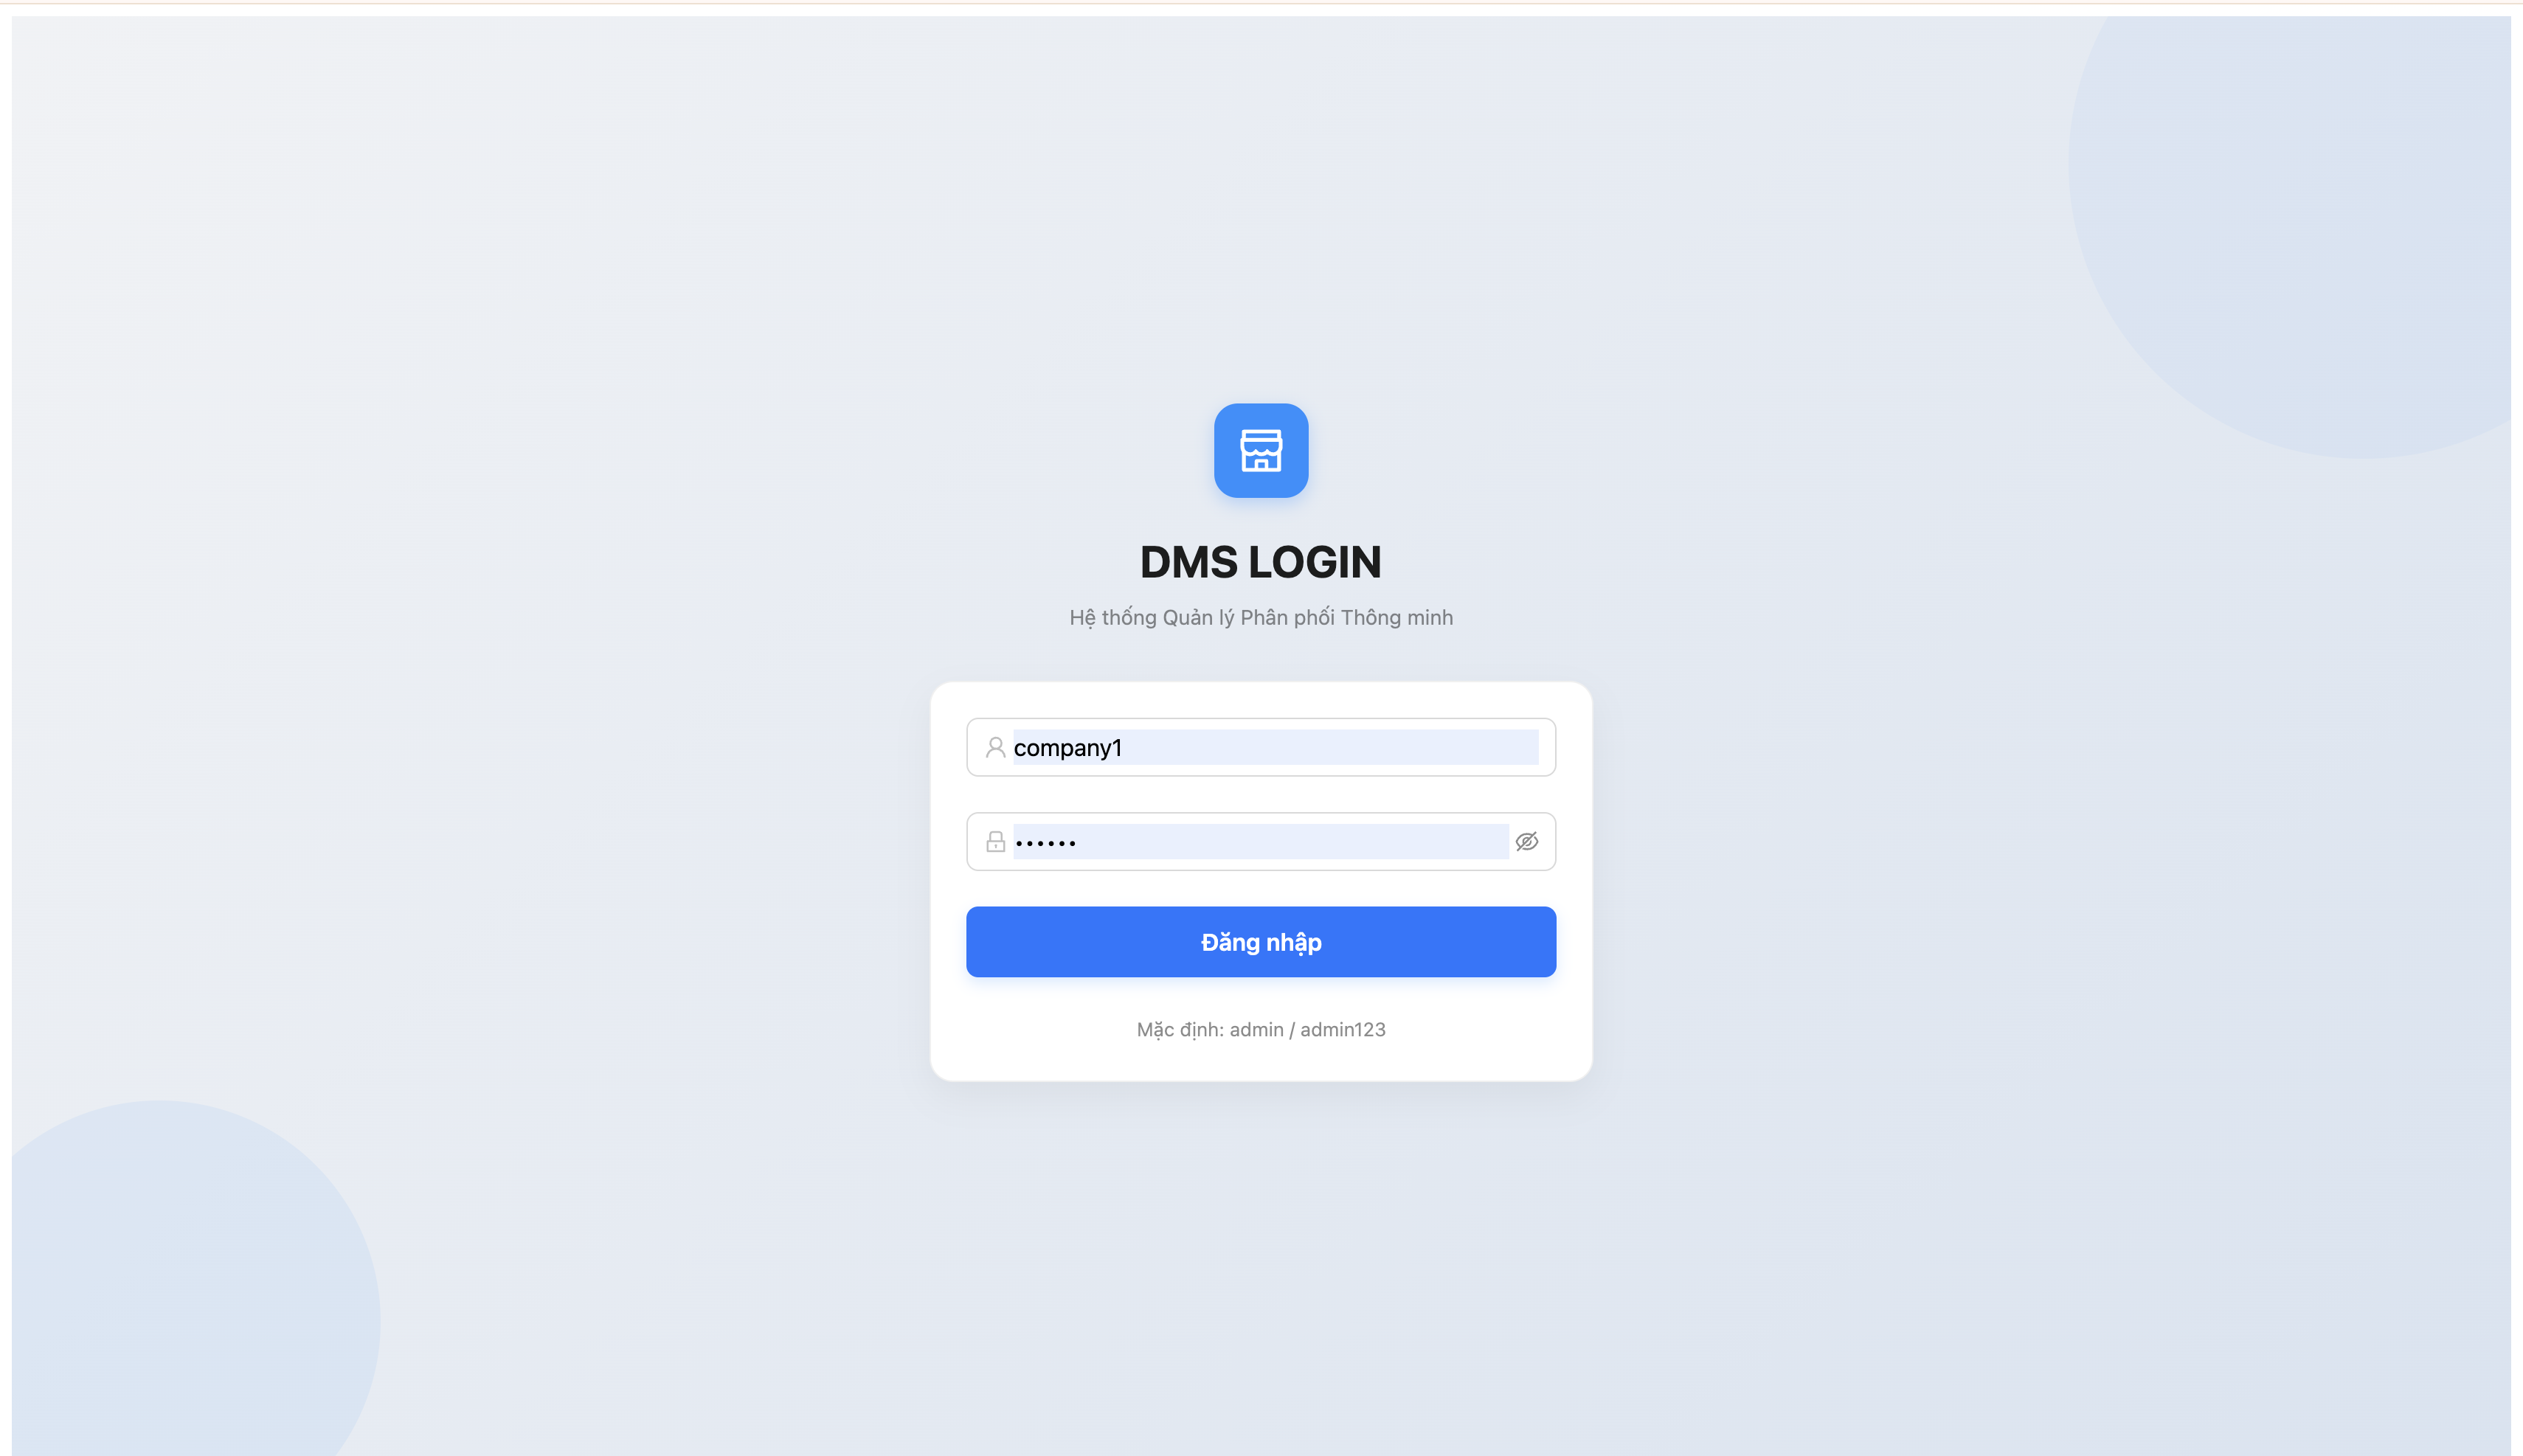
\includegraphics[width=0.62\linewidth]{Figure/screenshots/01-login.png}
\caption{Authentication screen}\label{fig:ui-login}
\end{figure}

Figure~\ref{fig:ui-login} shows the single sign-in screen through which every
user enters the system. Credentials submitted here are verified by the backend,
which returns a signed JSON Web Token that the browser then attaches to every
subsequent request; the routing and authorisation consequences of this token are
discussed in Section~\ref{sec:deployment}. Because all functional pages are
guarded, this screen is the only one reachable without a valid session.

\begin{figure}[H]\centering
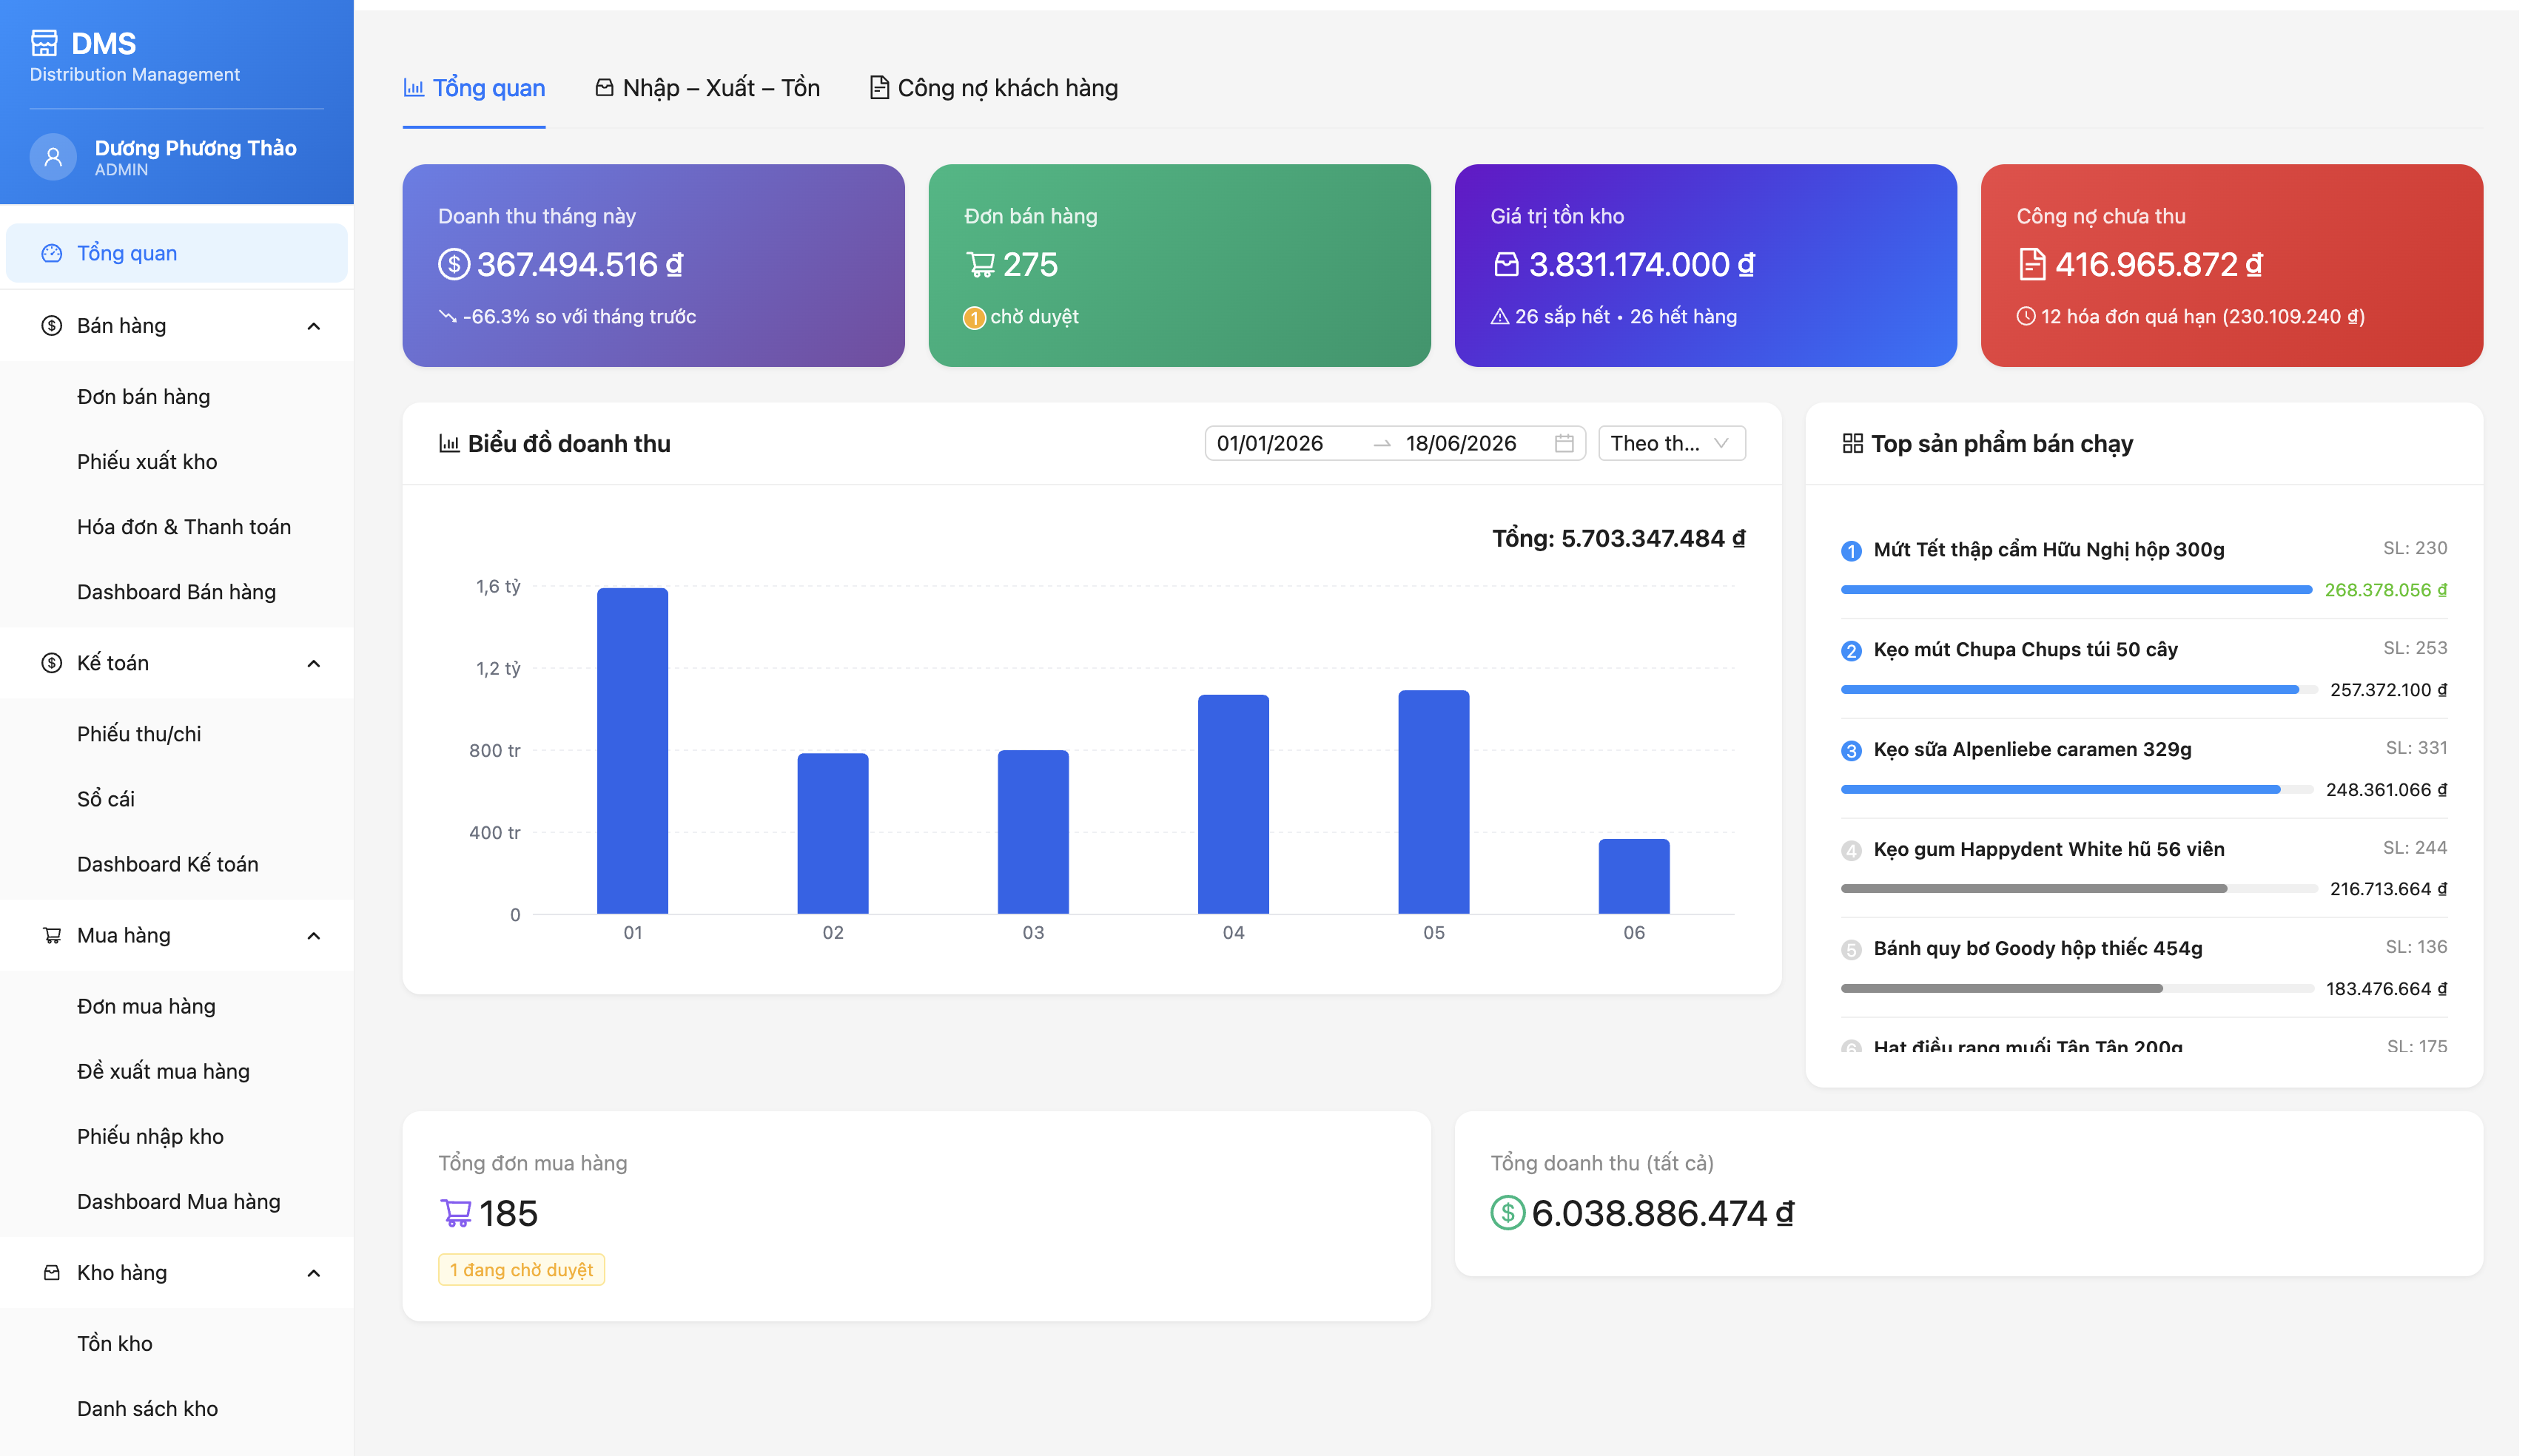
\includegraphics[width=0.95\linewidth]{Figure/screenshots/02-dashboard.png}
\caption{Management dashboard with aggregate indicators}\label{fig:ui-dashboard}
\end{figure}

Figure~\ref{fig:ui-dashboard} presents the management dashboard. Four
key-performance-indicator cards summarise (i) current-month revenue, (ii) the
number of sales orders, (iii) the total monetary value of stock on hand, and
(iv) outstanding accounts receivable, while a revenue chart and a
best-selling-product ranking give a quick operational overview. These figures are
aggregated on the server from the transactional tables rather than computed in
the browser, so the dashboard reflects the same data that drives the rest of the
application.

\begin{figure}[H]\centering
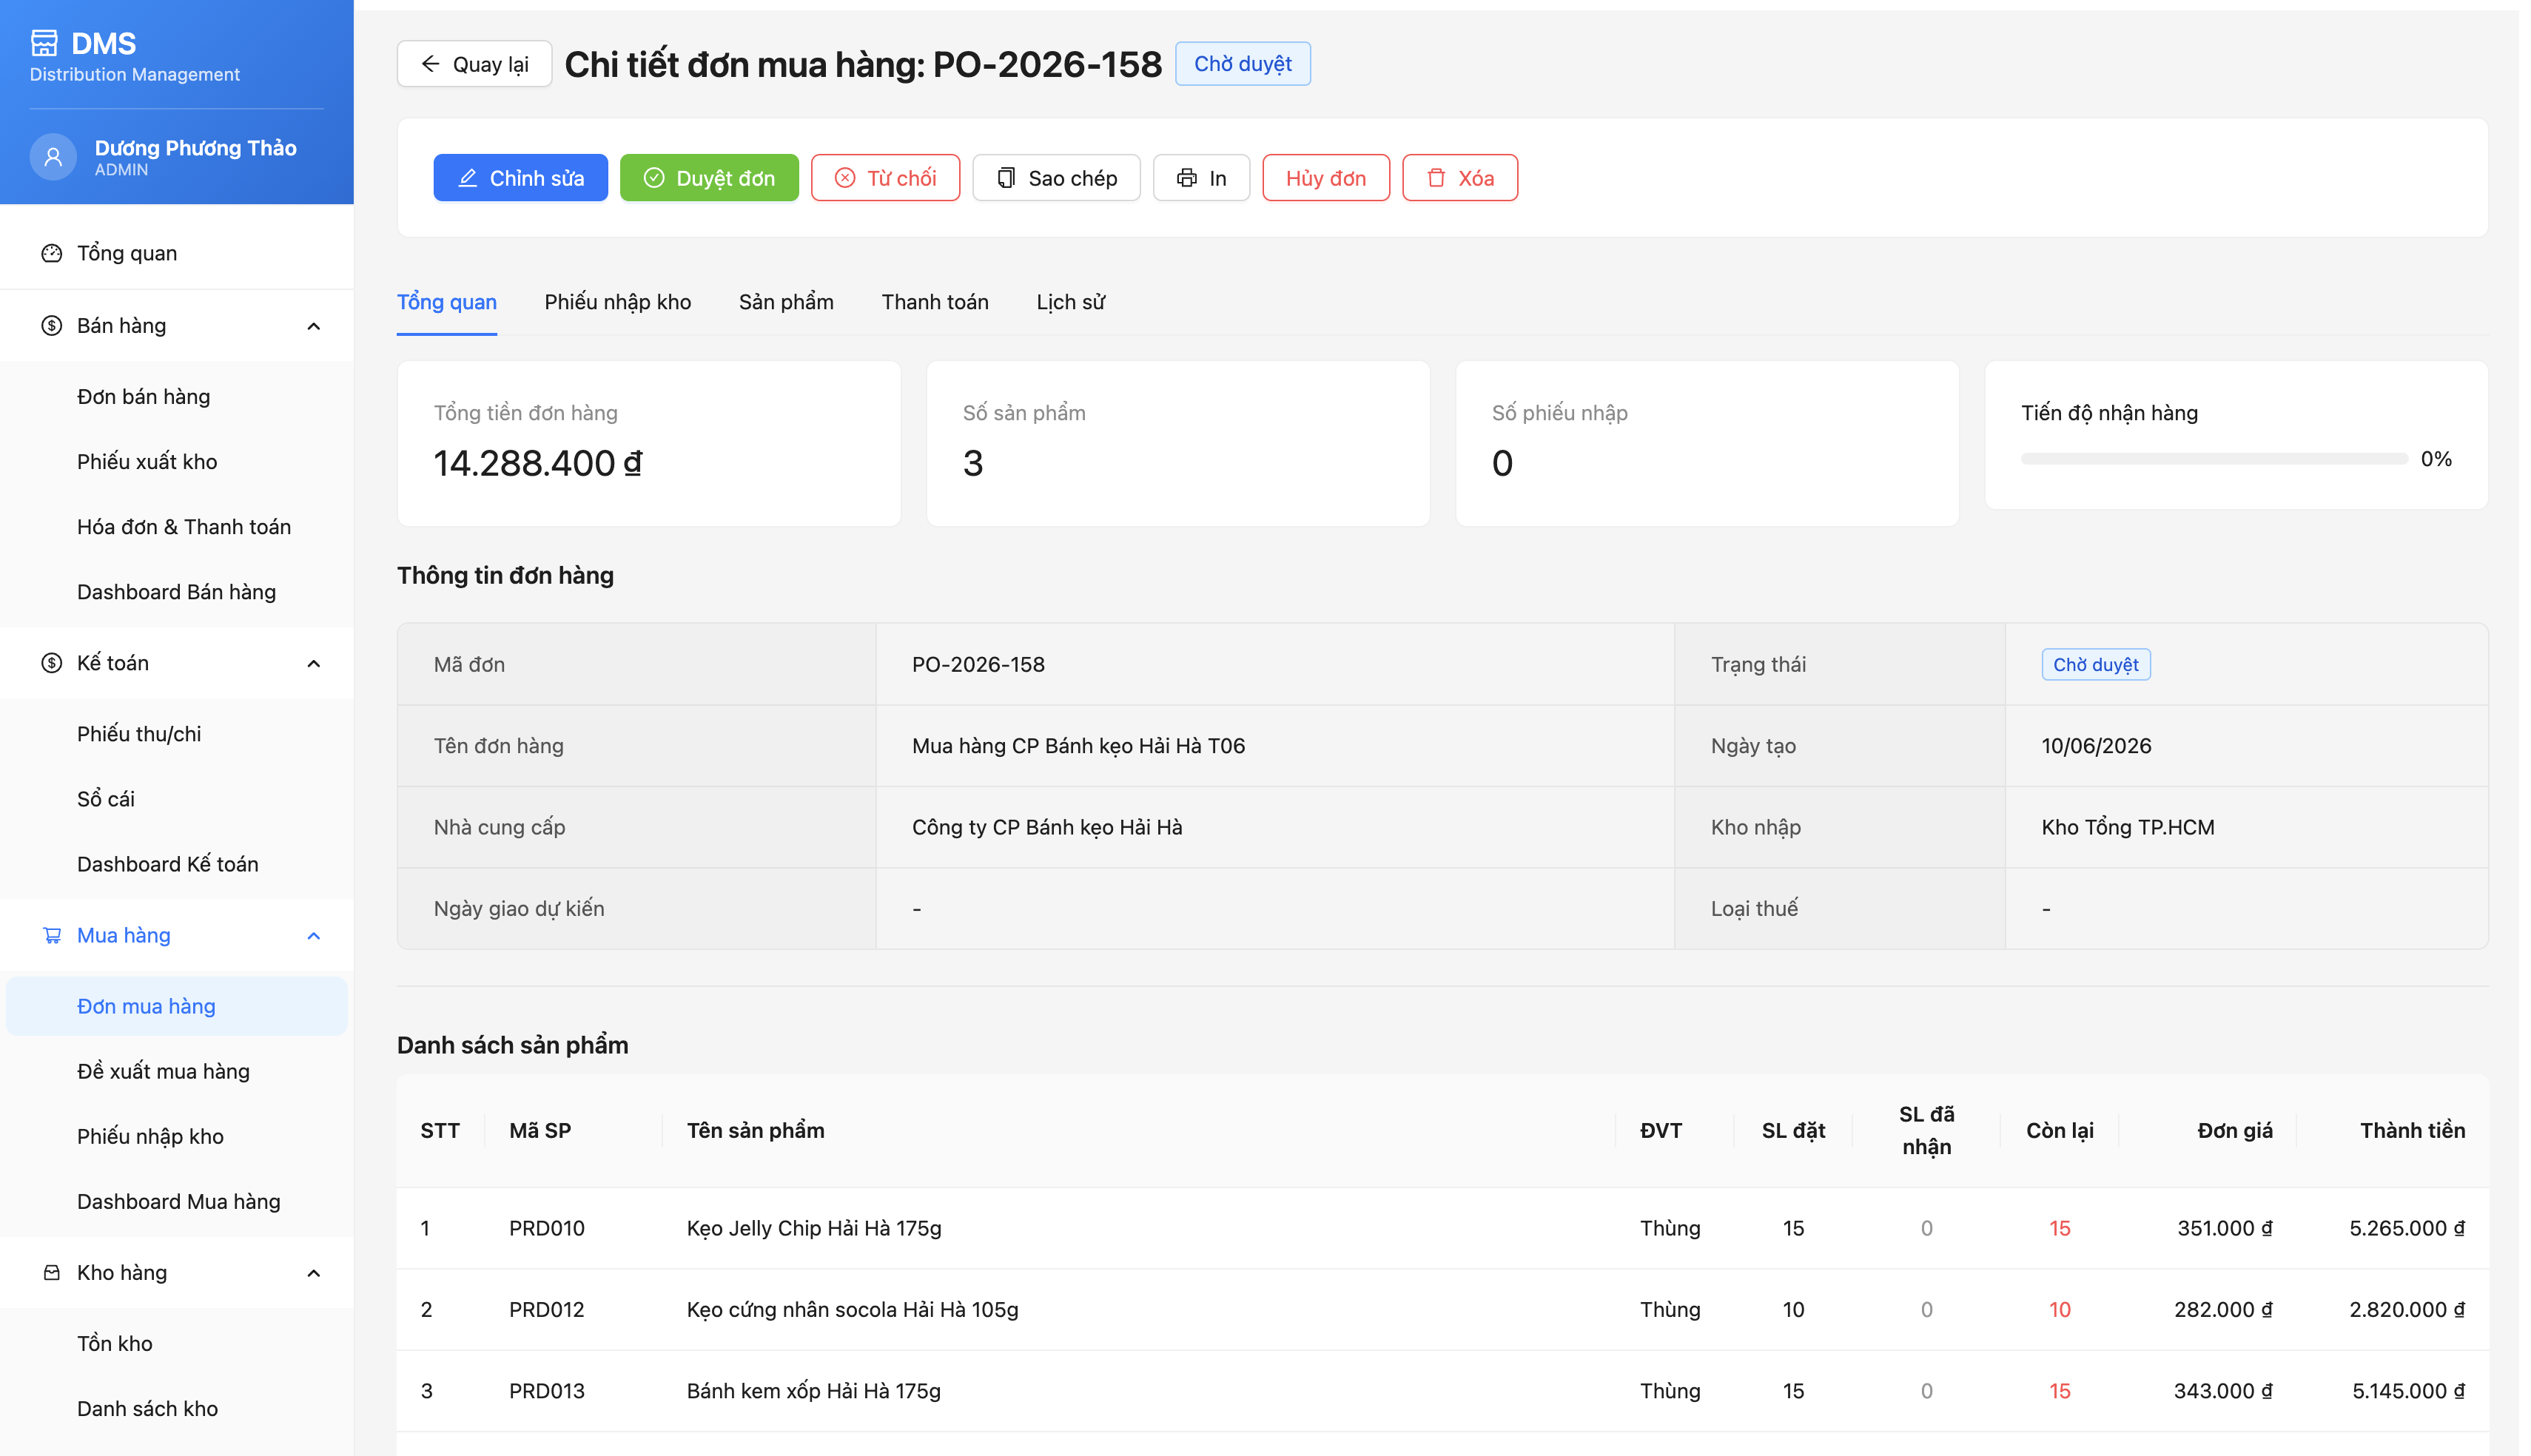
\includegraphics[width=0.95\linewidth]{Figure/screenshots/03-approve-po.png}
\caption{Purchase-order approval}\label{fig:ui-po}
\end{figure}

Figure~\ref{fig:ui-po} shows the detail of purchase order PO-2026-158 in the
pending-approval state, together with its supplier and three ordered lines. The
Approve action visible at the top transitions the order into an approved state
that authorises a subsequent goods receipt; rejecting or editing the order is
only permitted while it remains pending. This screen is the entry point of the
inbound flow.

\begin{figure}[H]\centering
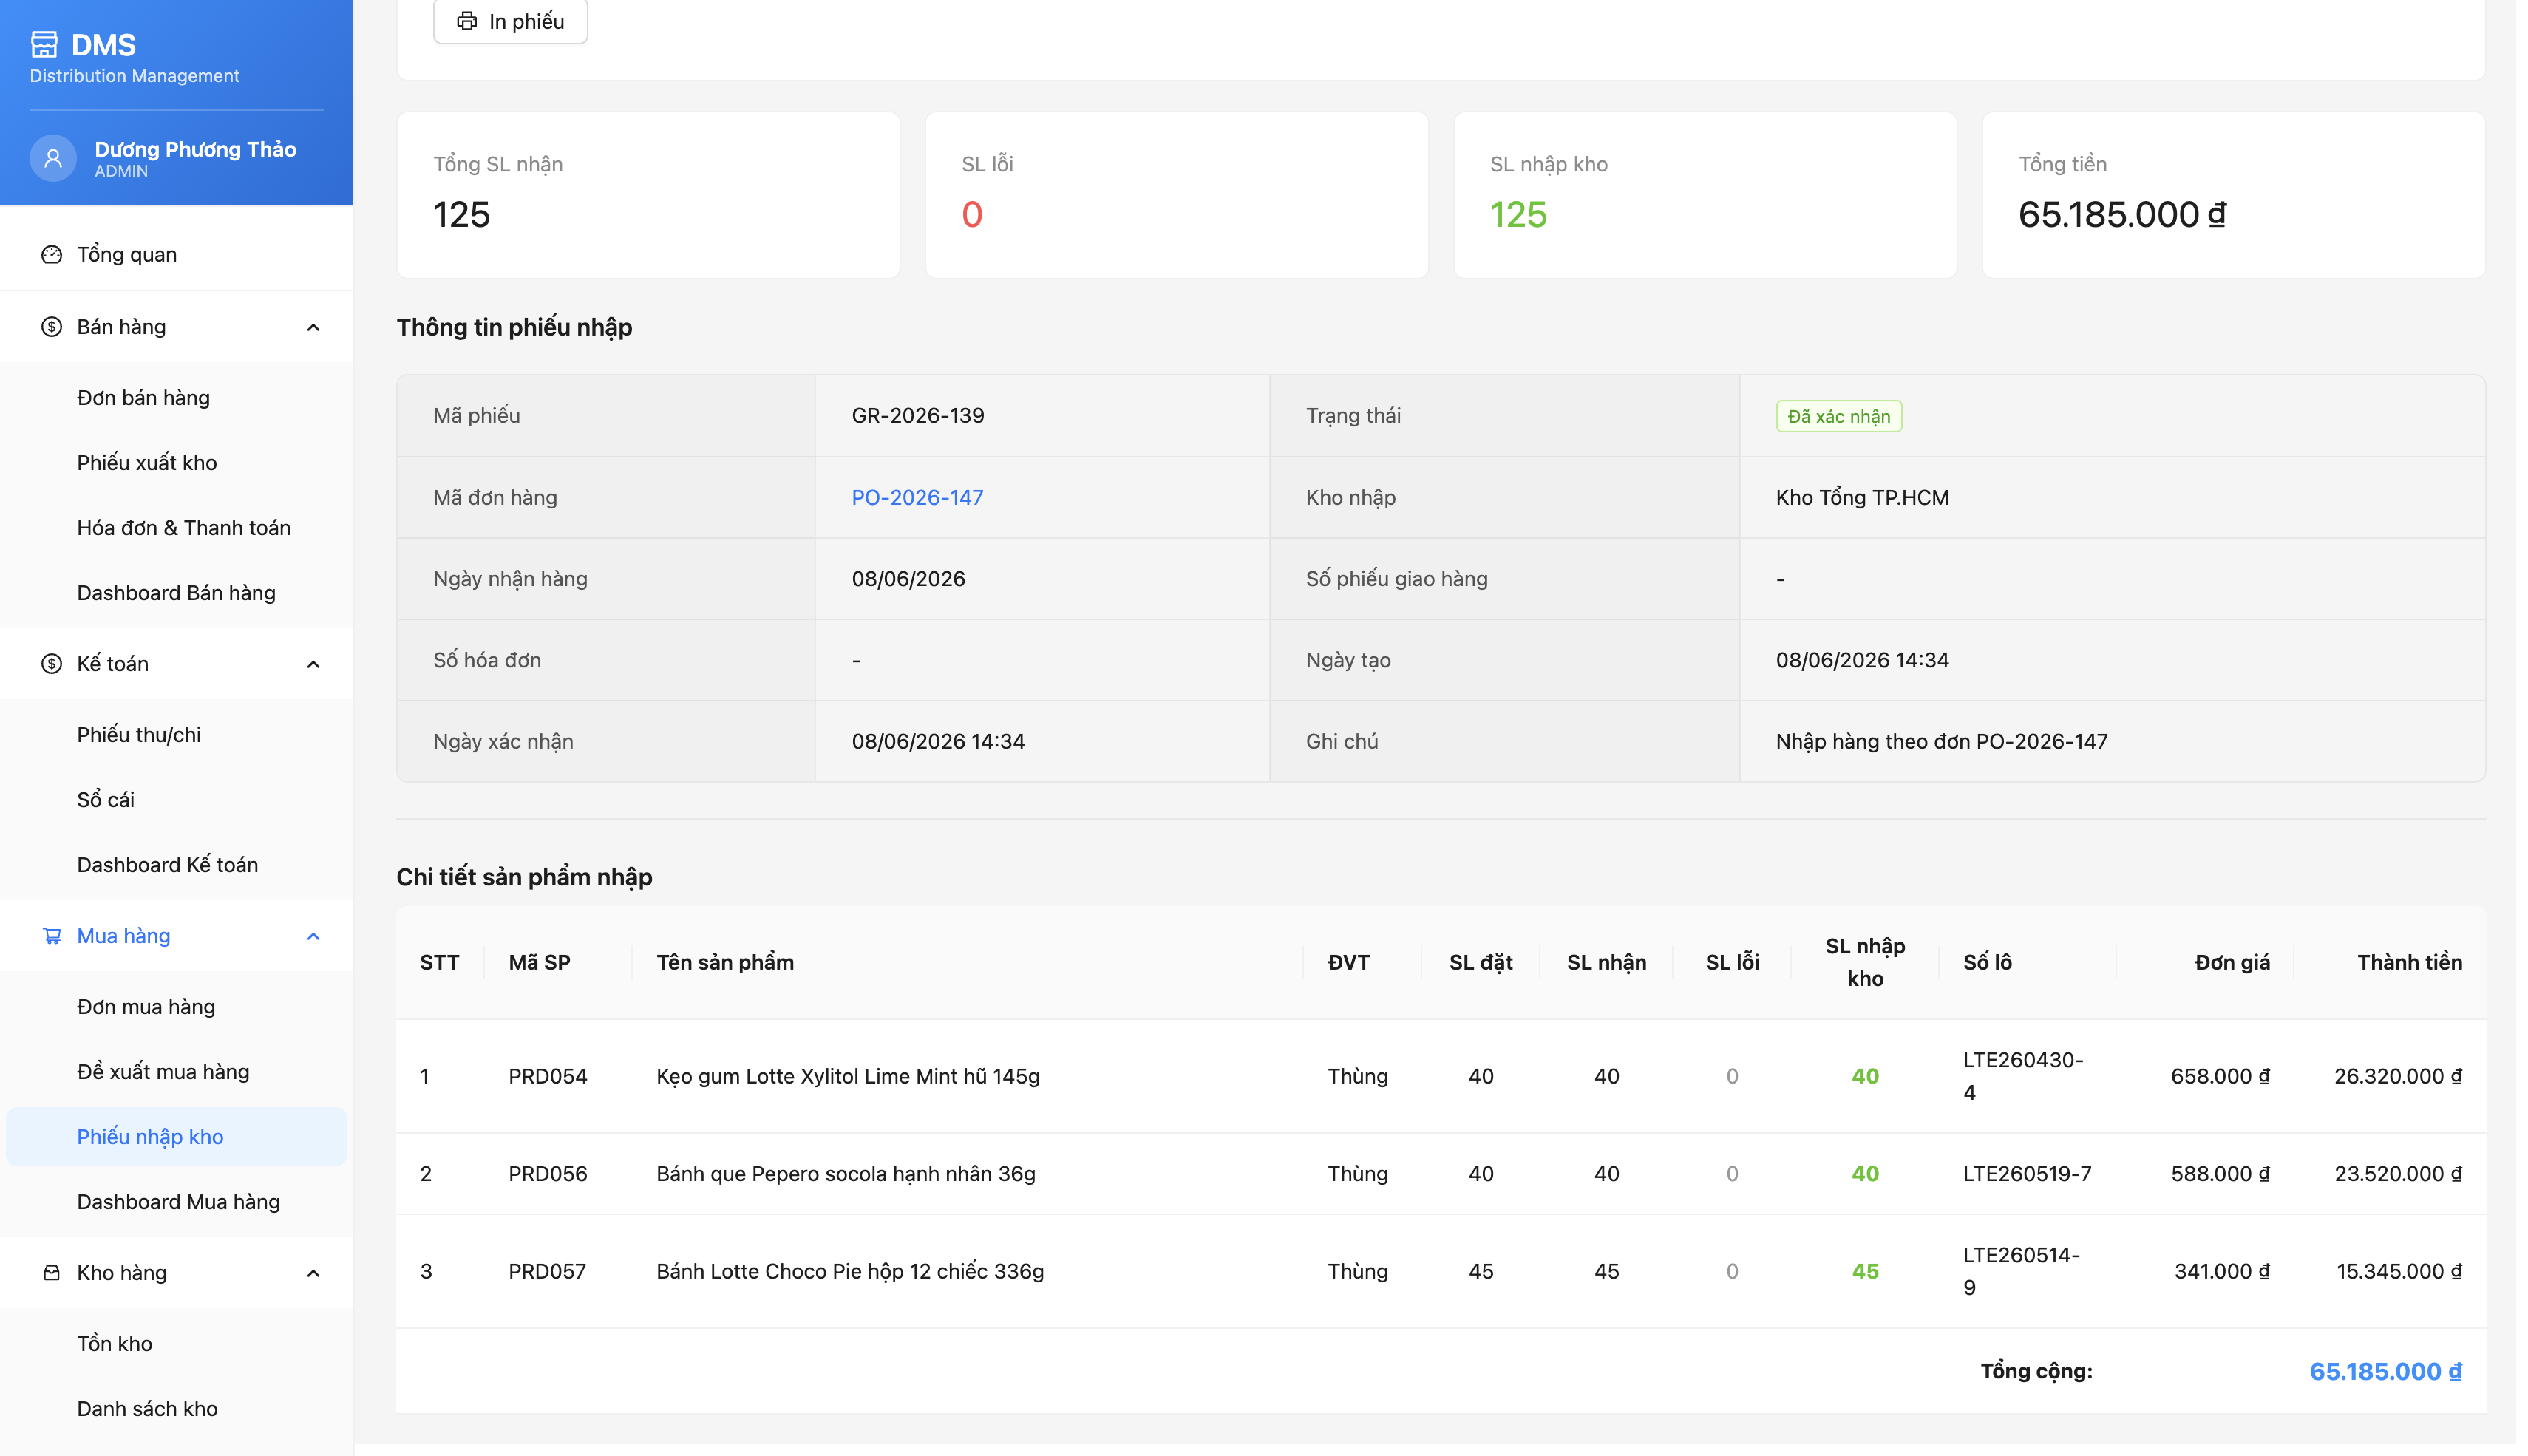
\includegraphics[width=0.95\linewidth]{Figure/screenshots/04-goods-receipt.png}
\caption{Goods-receipt confirmation with per-line lot numbers}\label{fig:ui-gr}
\end{figure}

Figure~\ref{fig:ui-gr} shows the confirmation of goods receipt GR-2026-139 against
purchase order PO-2026-147. Each received line is recorded against a distinct lot
number (for example LTE260430-4), and the accepted quantity is what is finally
added to stock. It is at this point that batch identity enters the system, which
is the precondition for the first-expired-first-out issuing illustrated later in
Figure~\ref{fig:ui-gi} and detailed in the sequence diagram of
Figure~\ref{fig:seq-fefo}.

\begin{figure}[H]\centering
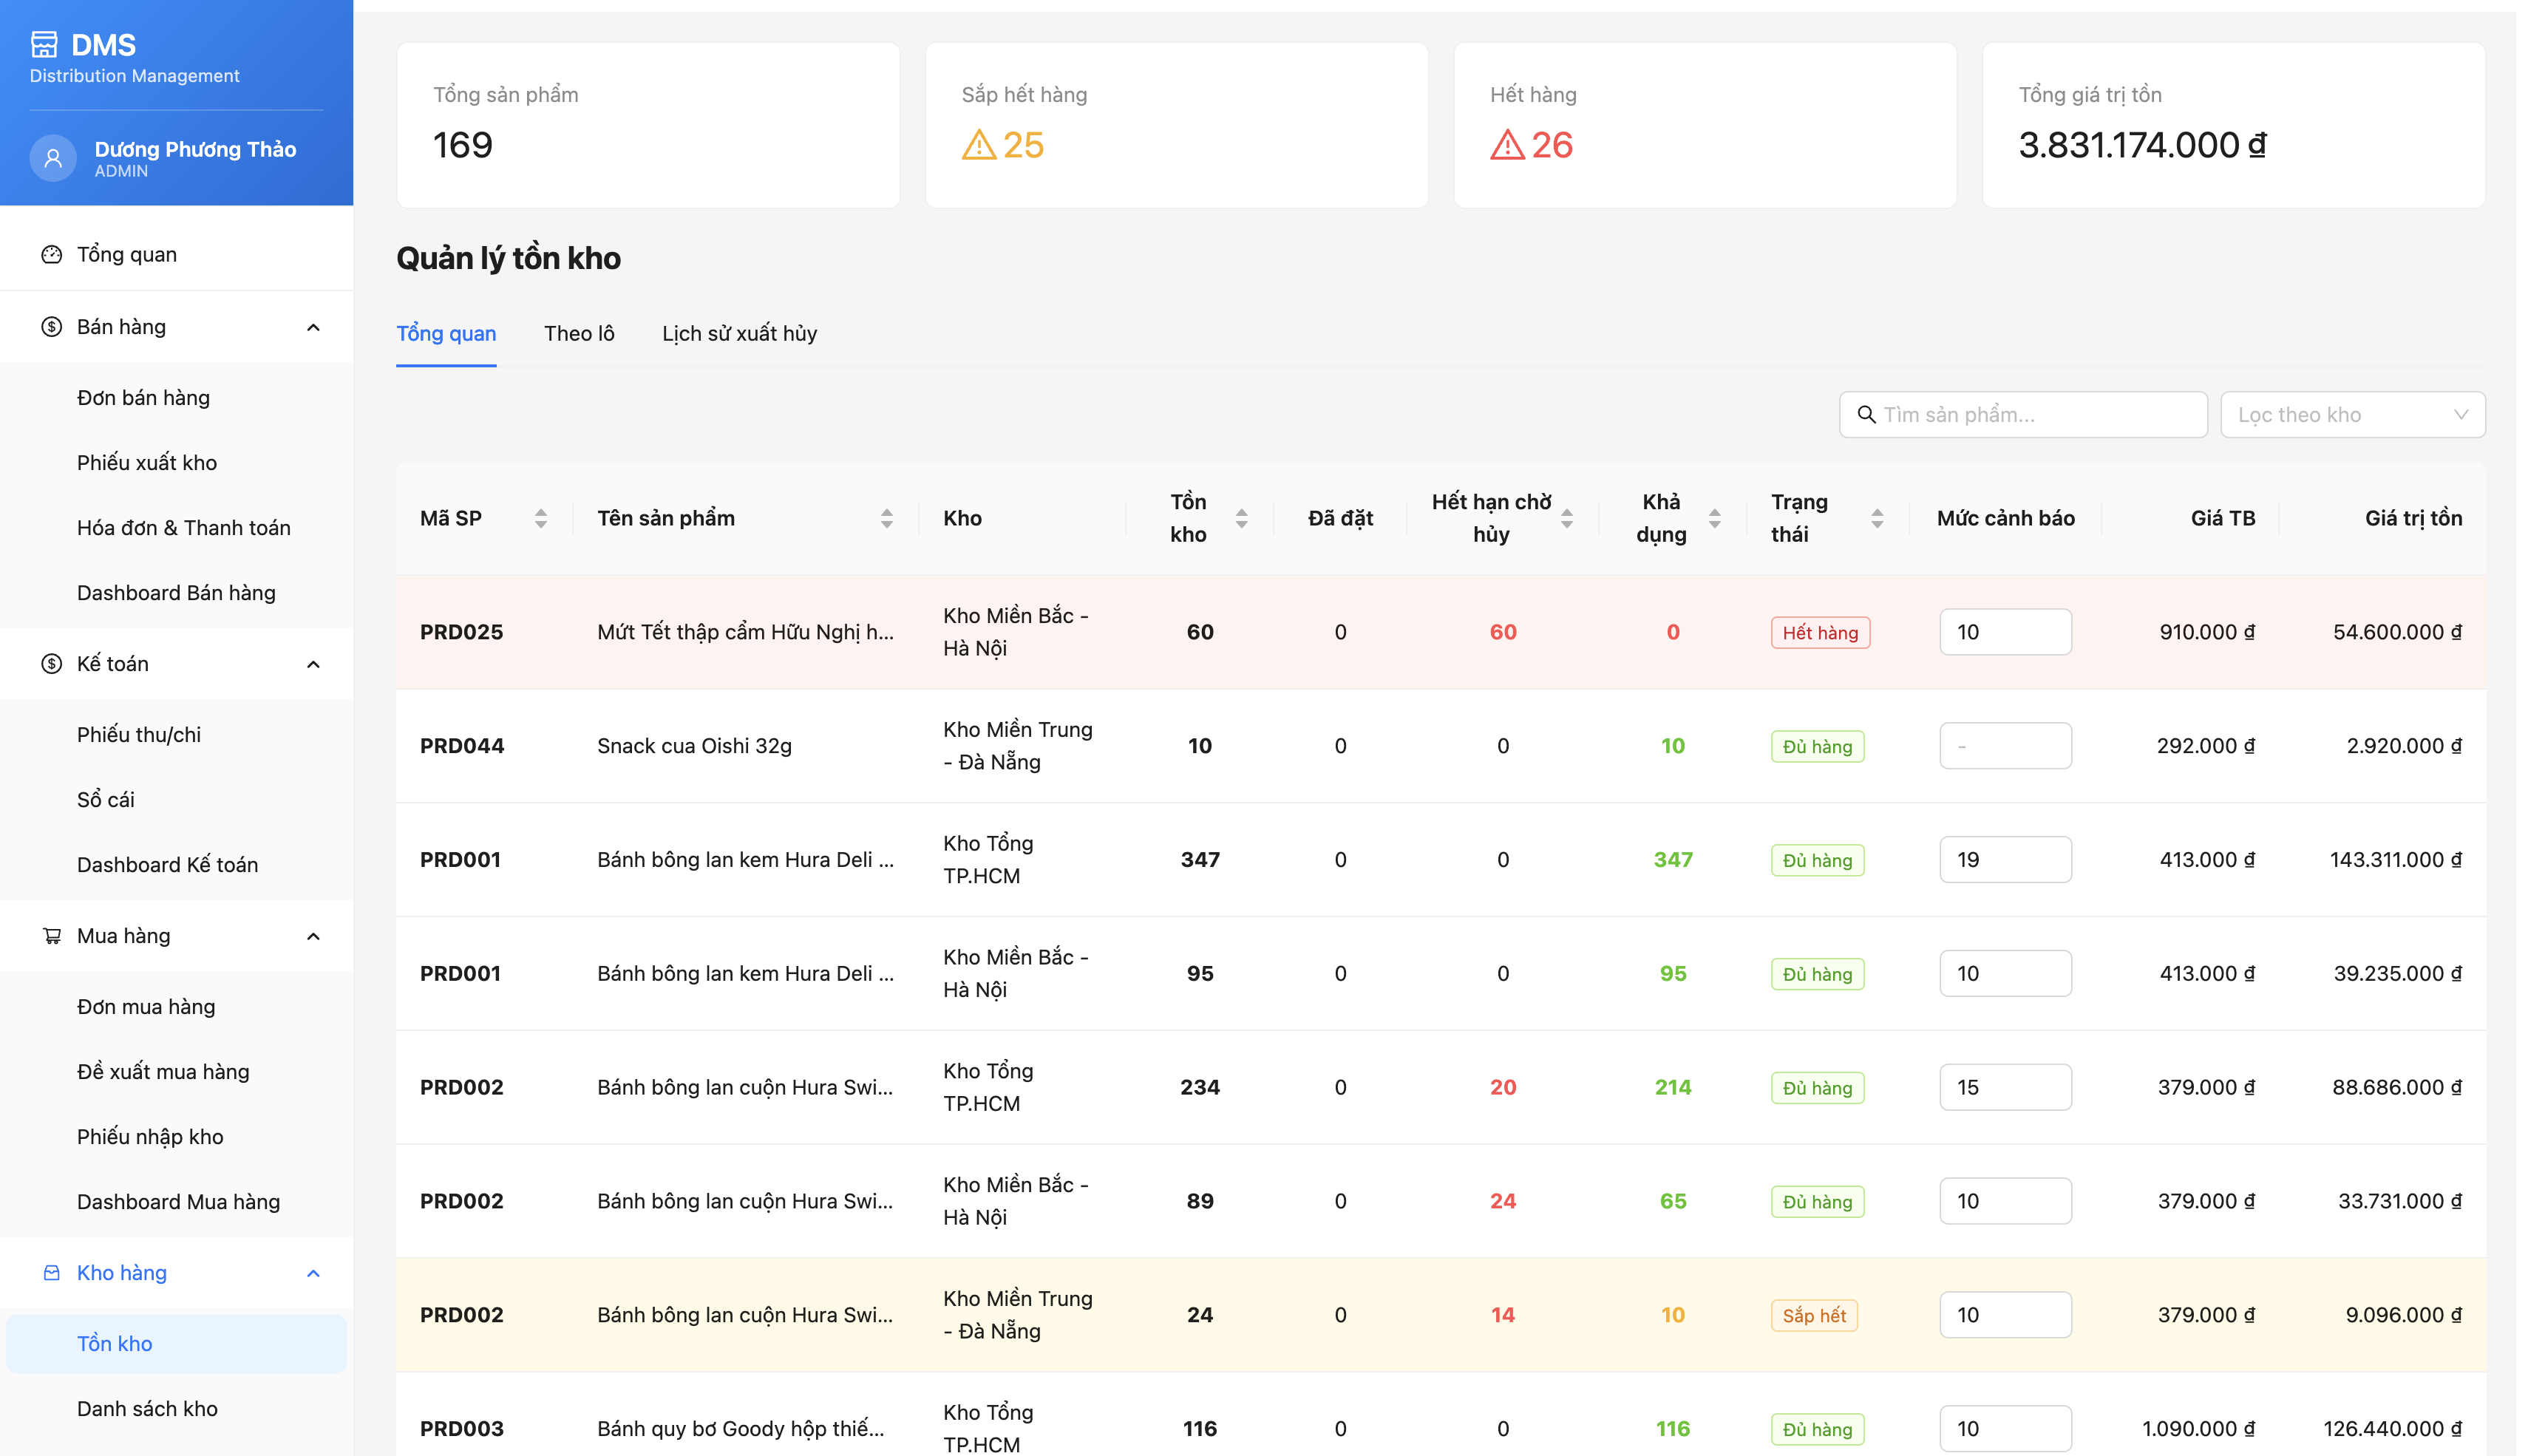
\includegraphics[width=0.95\linewidth]{Figure/screenshots/05-inventory-by-lot.png}
\caption{Inventory overview: on-hand, reserved, available and expiry-pending
quantities per product and warehouse}\label{fig:ui-inventory}
\end{figure}

Figure~\ref{fig:ui-inventory} shows the inventory overview. For each
product-warehouse pair the table separates quantity on hand, reserved quantity,
quantity pending disposal because of expiry, and available quantity, and assigns
a status tag such as in-stock, low-stock, or out-of-stock. This separation is the
on-screen manifestation of the reservation mechanism: the available quantity is
computed as the quantity on hand minus the reserved quantity, and it is this
available figure, not the raw on-hand figure, that is checked when a sales order
is approved. Confirming a goods issue is what finally lowers the on-hand quantity.

\begin{figure}[H]\centering
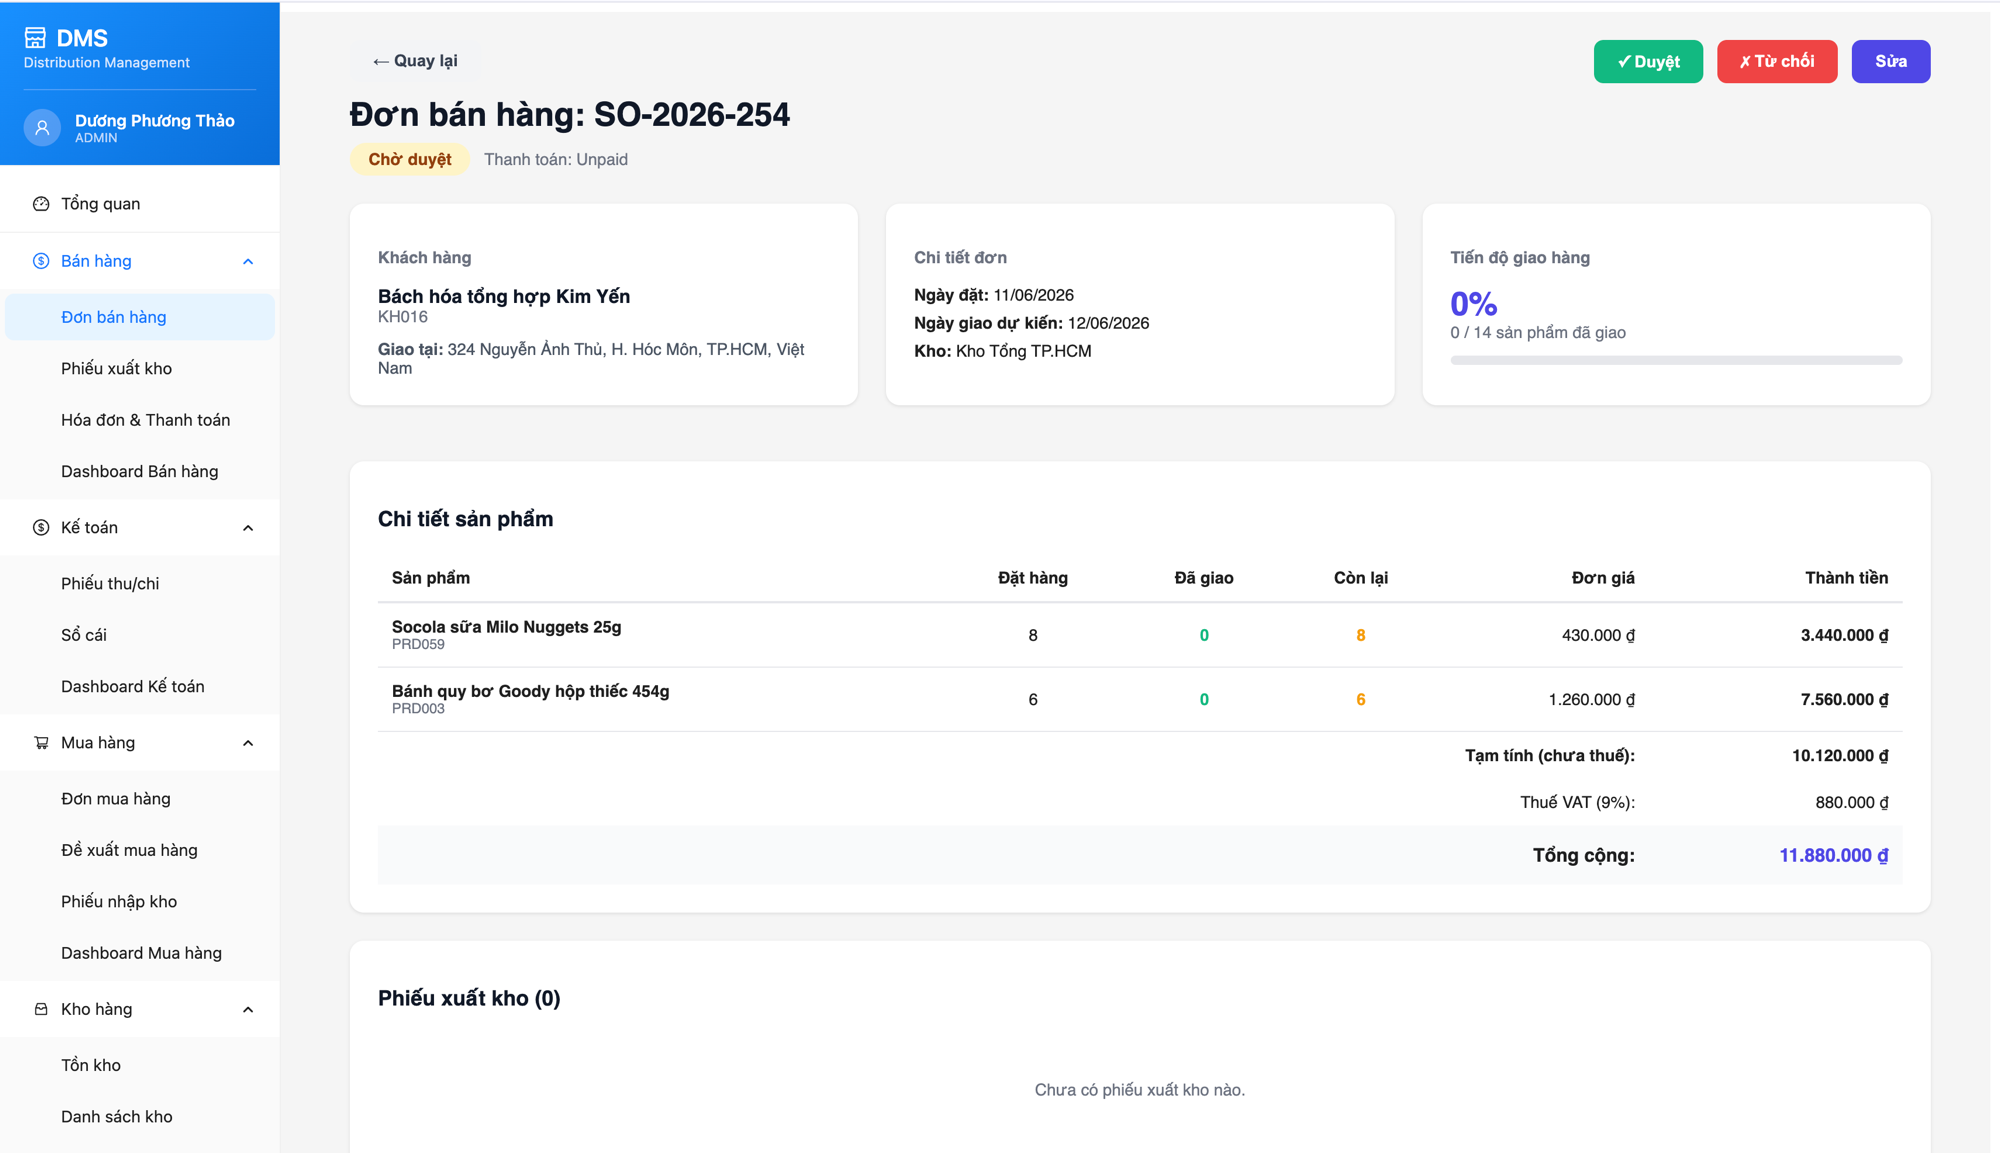
\includegraphics[width=0.95\linewidth]{Figure/screenshots/06-approve-so.png}
\caption{Sales-order approval, the point at which available stock is checked and
reserved}\label{fig:ui-so}
\end{figure}

Figure~\ref{fig:ui-so} shows sales order SO-2026-254 in the pending-approval
state, with its customer, two ordered lines, and the computed subtotal, value-added
tax, and total. Approval is the decisive step in the outbound flow: when the
Approve action is invoked, the server checks that sufficient available stock
exists for every line and, if so, reserves exactly the ordered quantity before
moving the order to the approved state. This is where the available-quantity logic
visible in Figure~\ref{fig:ui-inventory} is enforced, so that two orders competing
for the same stock cannot both be approved beyond what is physically on hand. The
delivery-progress indicator remains at zero per cent until the corresponding goods
issue is confirmed.

\begin{figure}[H]\centering
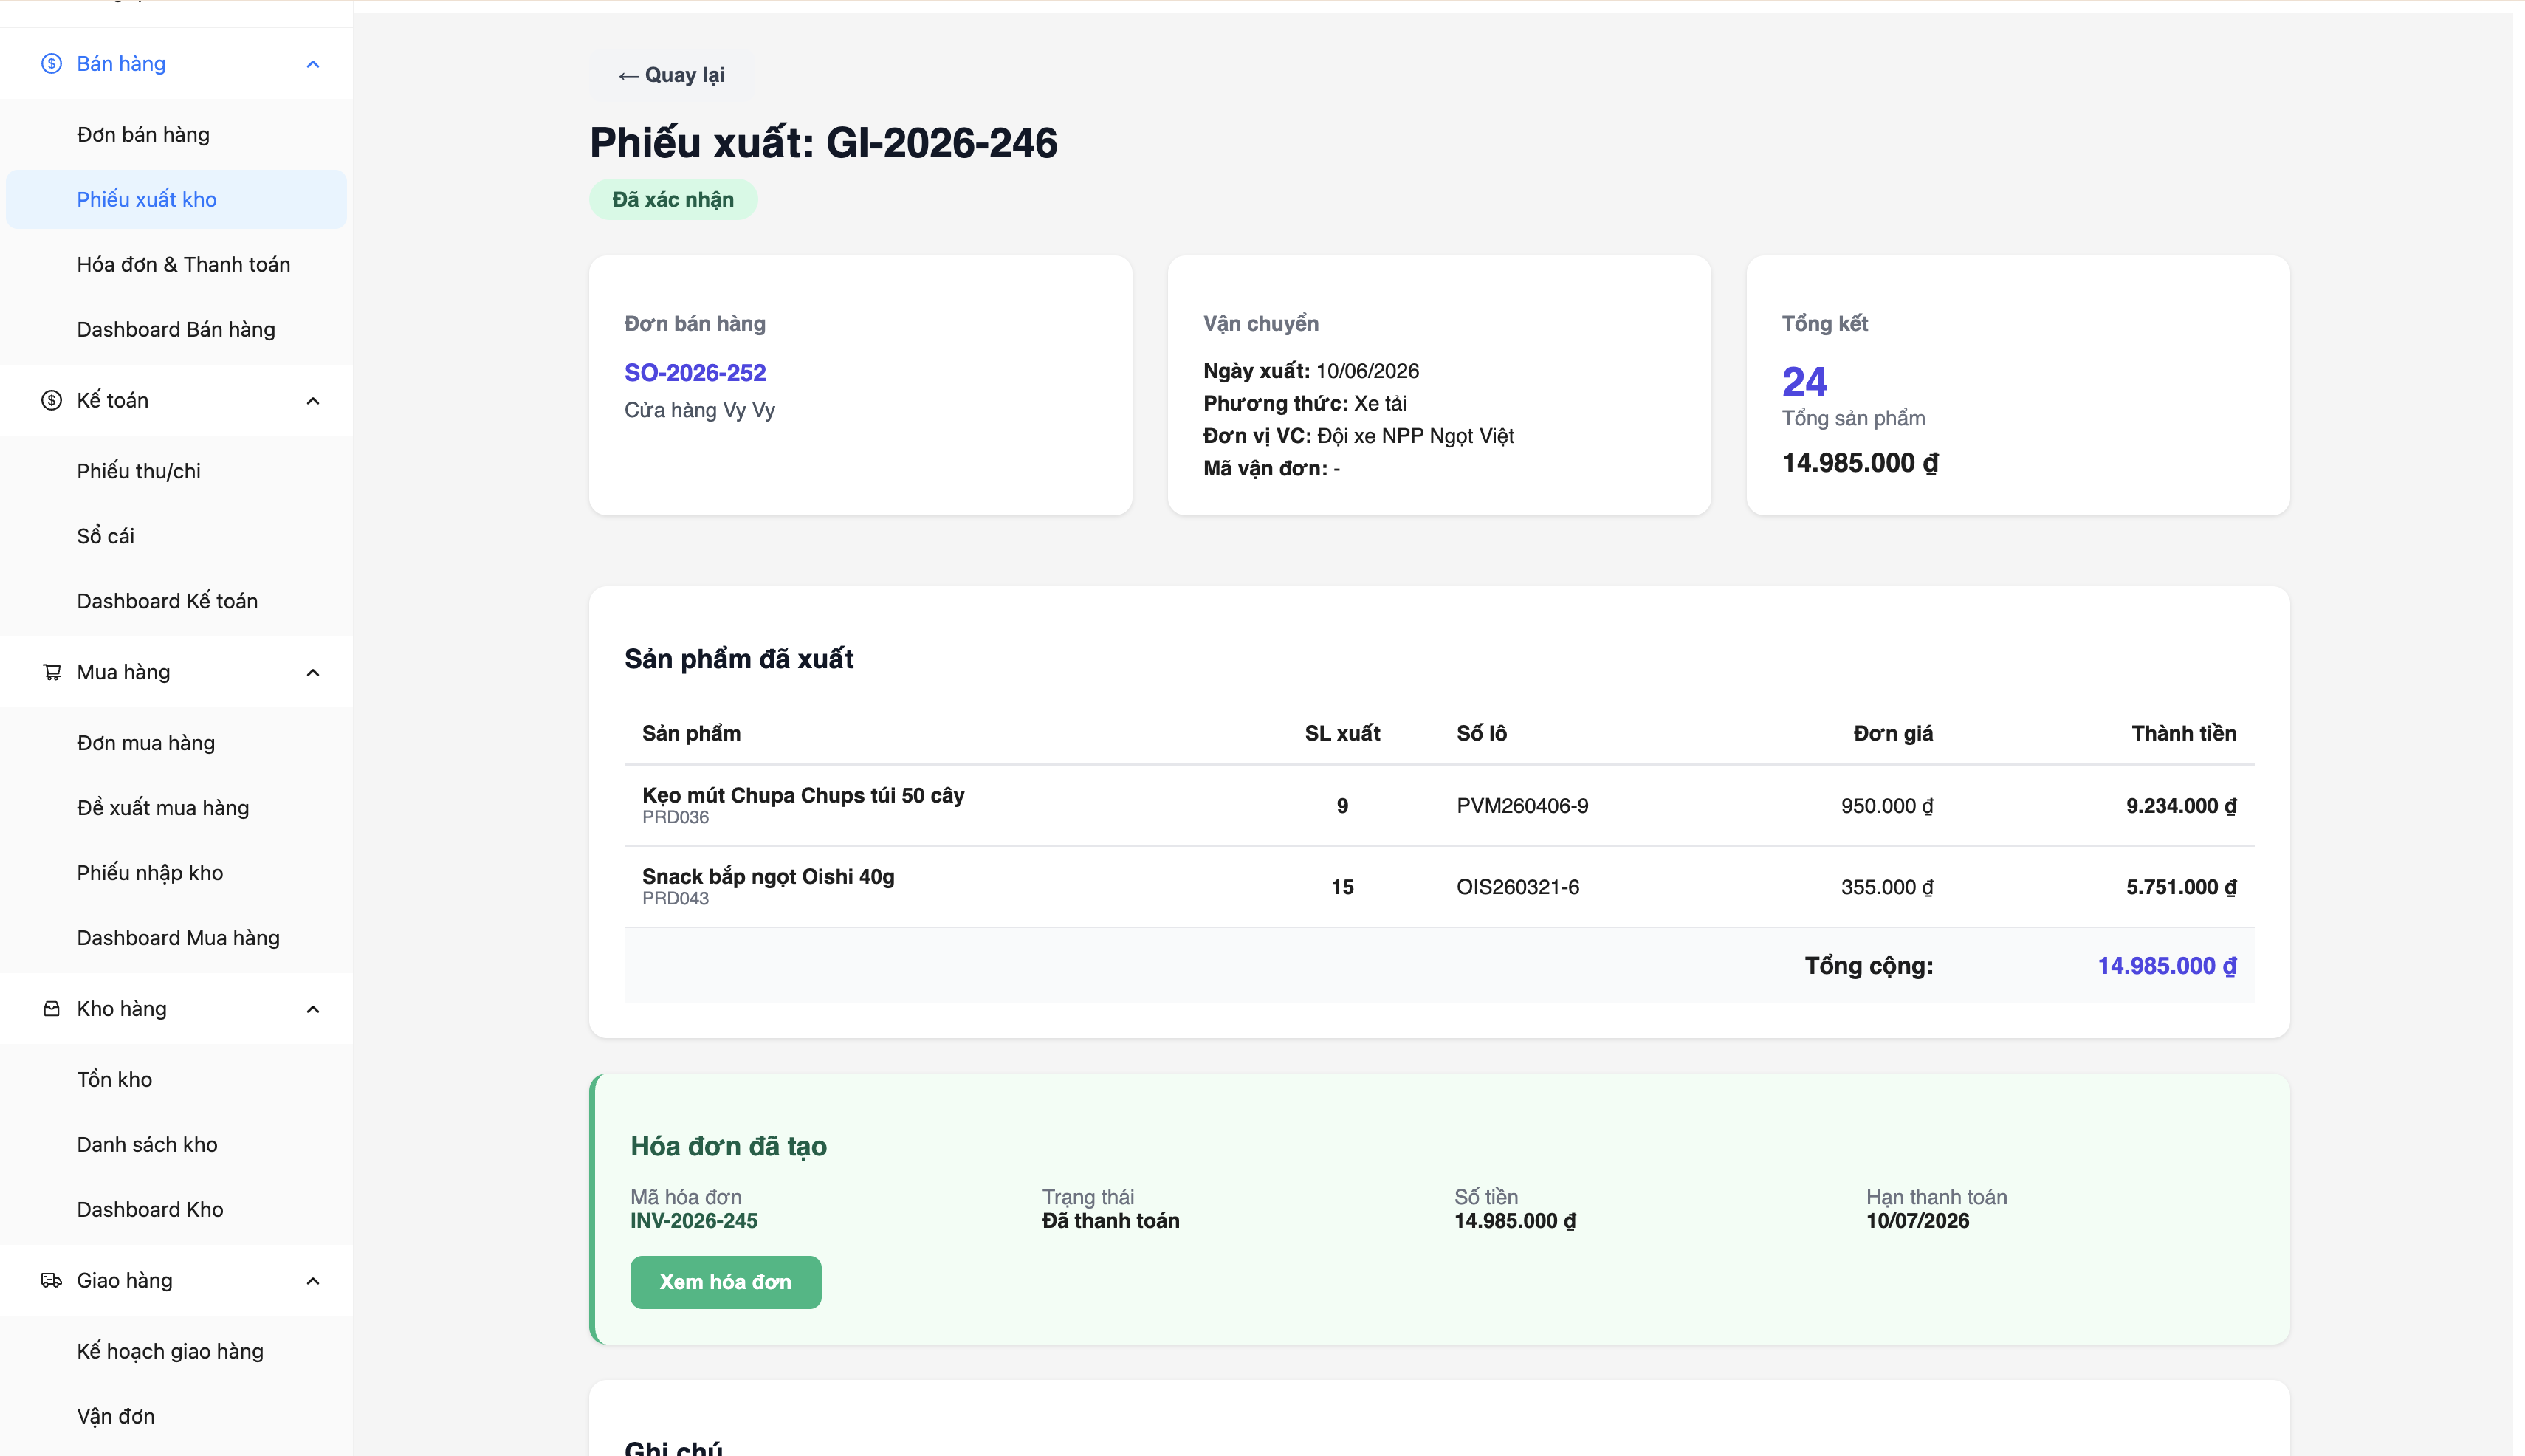
\includegraphics[width=0.95\linewidth]{Figure/screenshots/07-goods-issue-fefo.png}
\caption{Goods-issue confirmation with FEFO lot allocation}\label{fig:ui-gi}
\end{figure}

Figure~\ref{fig:ui-gi} shows the confirmation of goods issue GI-2026-246, which
fulfils sales order SO-2026-252. Each issued line is annotated with the specific
lot consumed (for example PVM260406-9), and these lots are the earliest-expiring
ones available, selected automatically by the FEFO allocation query rather than
chosen by the operator. The same panel shows that sales invoice INV-2026-245 is
generated automatically once the issue is confirmed, linking the warehouse and
accounting subsystems in a single transaction.

\begin{figure}[H]\centering
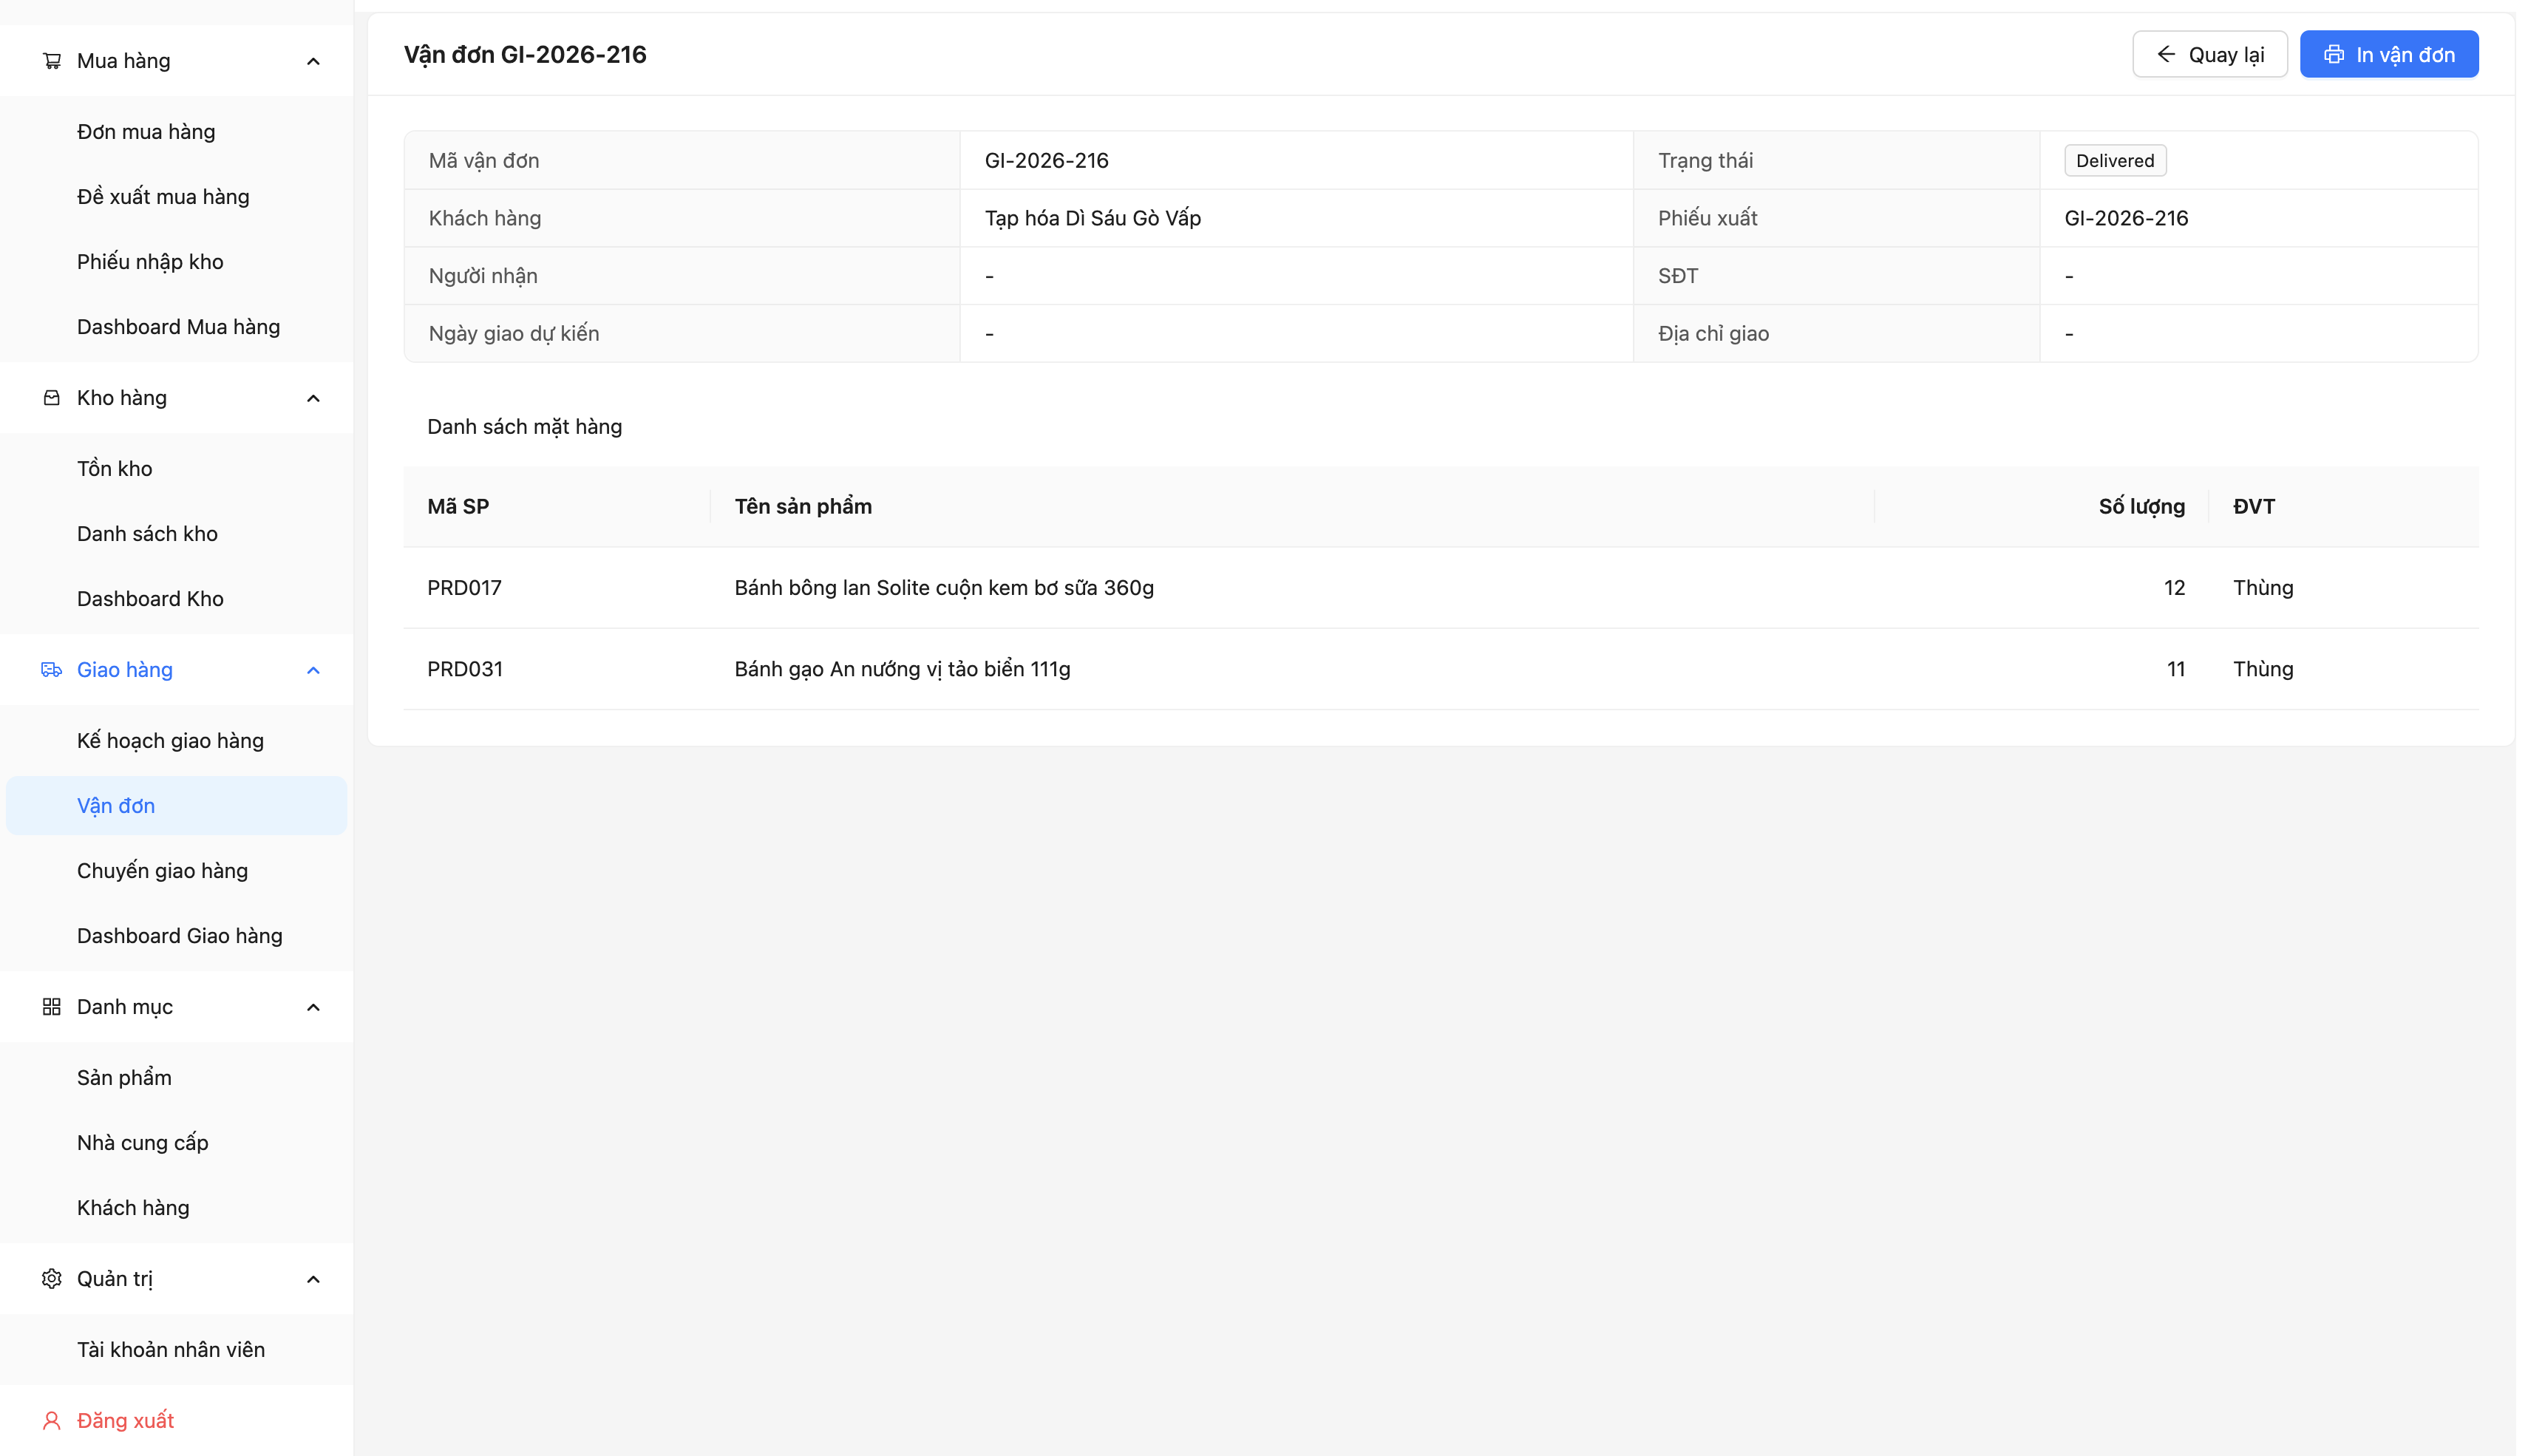
\includegraphics[width=0.95\linewidth]{Figure/screenshots/08-delivery-waybill.png}
\caption{Delivery waybill in the delivered state}\label{fig:ui-waybill}
\end{figure}

Figure~\ref{fig:ui-waybill} shows the waybill associated with issue GI-2026-216
after the trip has been completed, with its status set to delivered and the two
product lines to be handed to the customer. A printable version of this document
accompanies the driver; when a delivery fails instead of completing, the
corresponding stock is returned to inventory through the failed-delivery recovery
path discussed in Chapter~\ref{chapter:Contribution}.

\begin{figure}[H]\centering
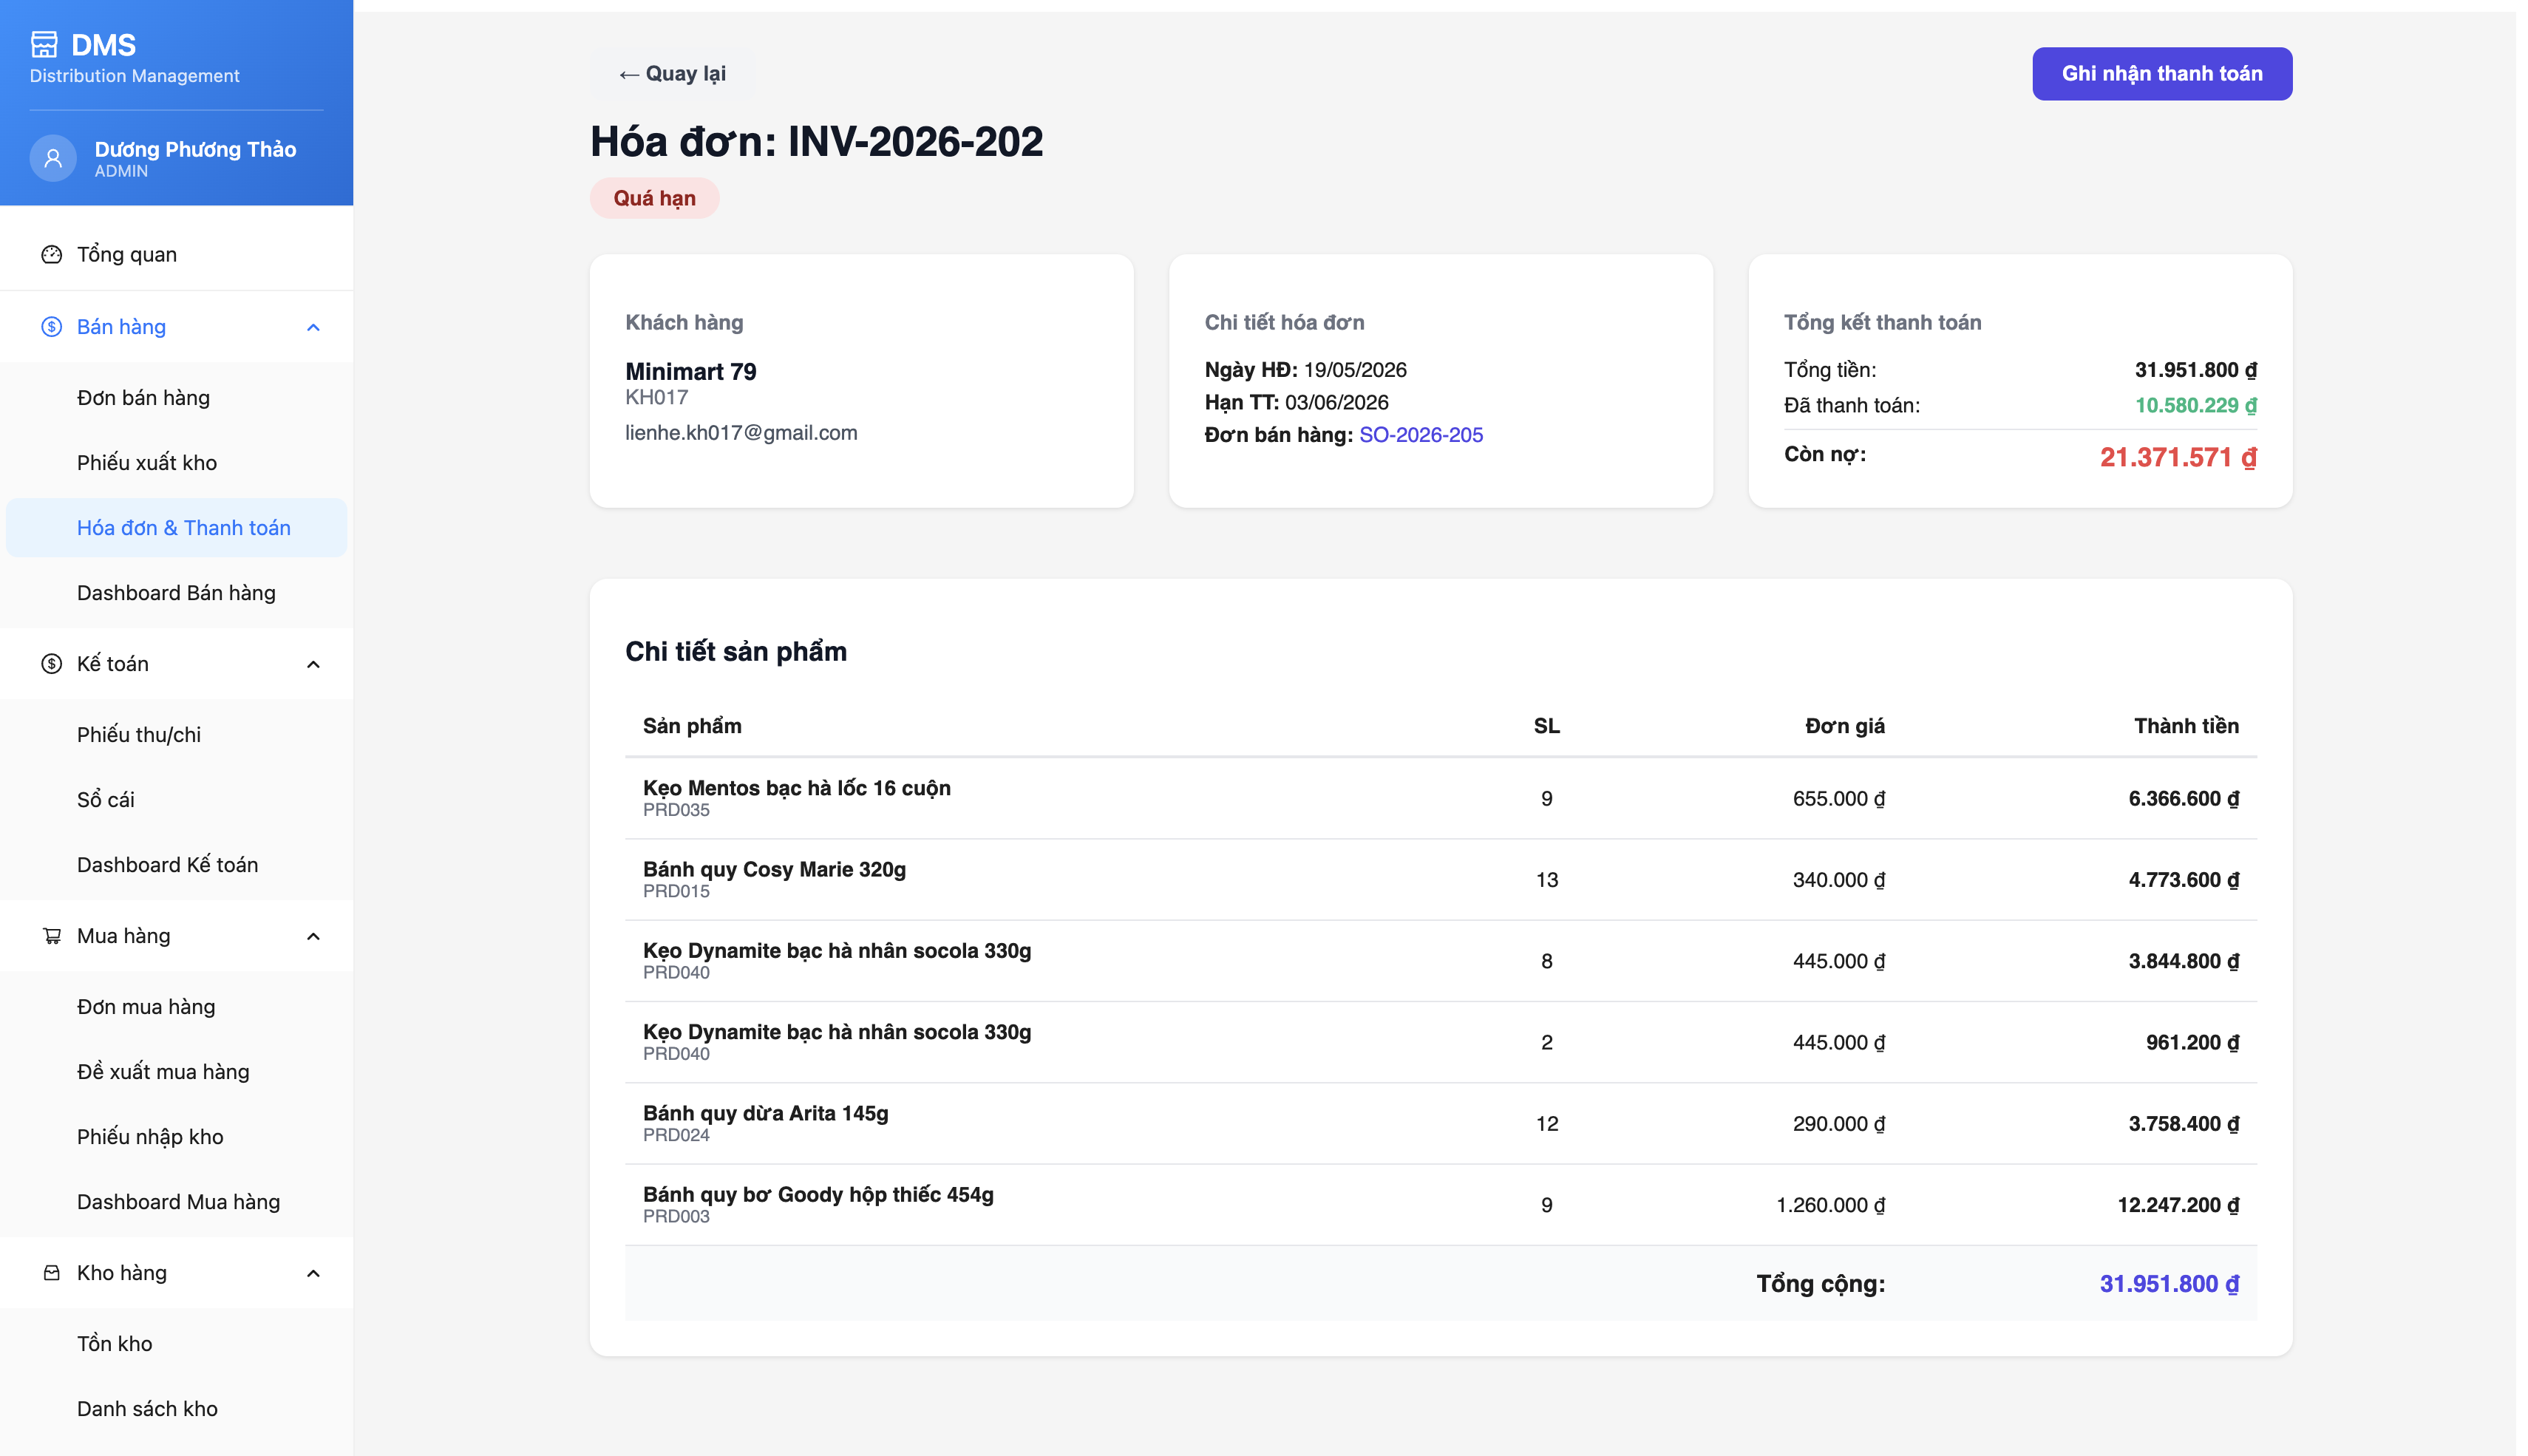
\includegraphics[width=0.95\linewidth]{Figure/screenshots/09-invoice.png}
\caption{Sales-invoice detail with partial settlement}\label{fig:ui-invoice}
\end{figure}

Figure~\ref{fig:ui-invoice} shows sales invoice INV-2026-202, issued to customer
Minimart~79 from sales order SO-2026-205. The invoice is only partially settled:
of a total of 31{,}951{,}800~VND, 10{,}580{,}229~VND has been received, leaving
21{,}371{,}571~VND outstanding, and the invoice is consequently flagged as
overdue. This partial-payment state is what the receivables ledger in
Figure~\ref{fig:ui-ledger} reconciles.

\begin{figure}[H]\centering
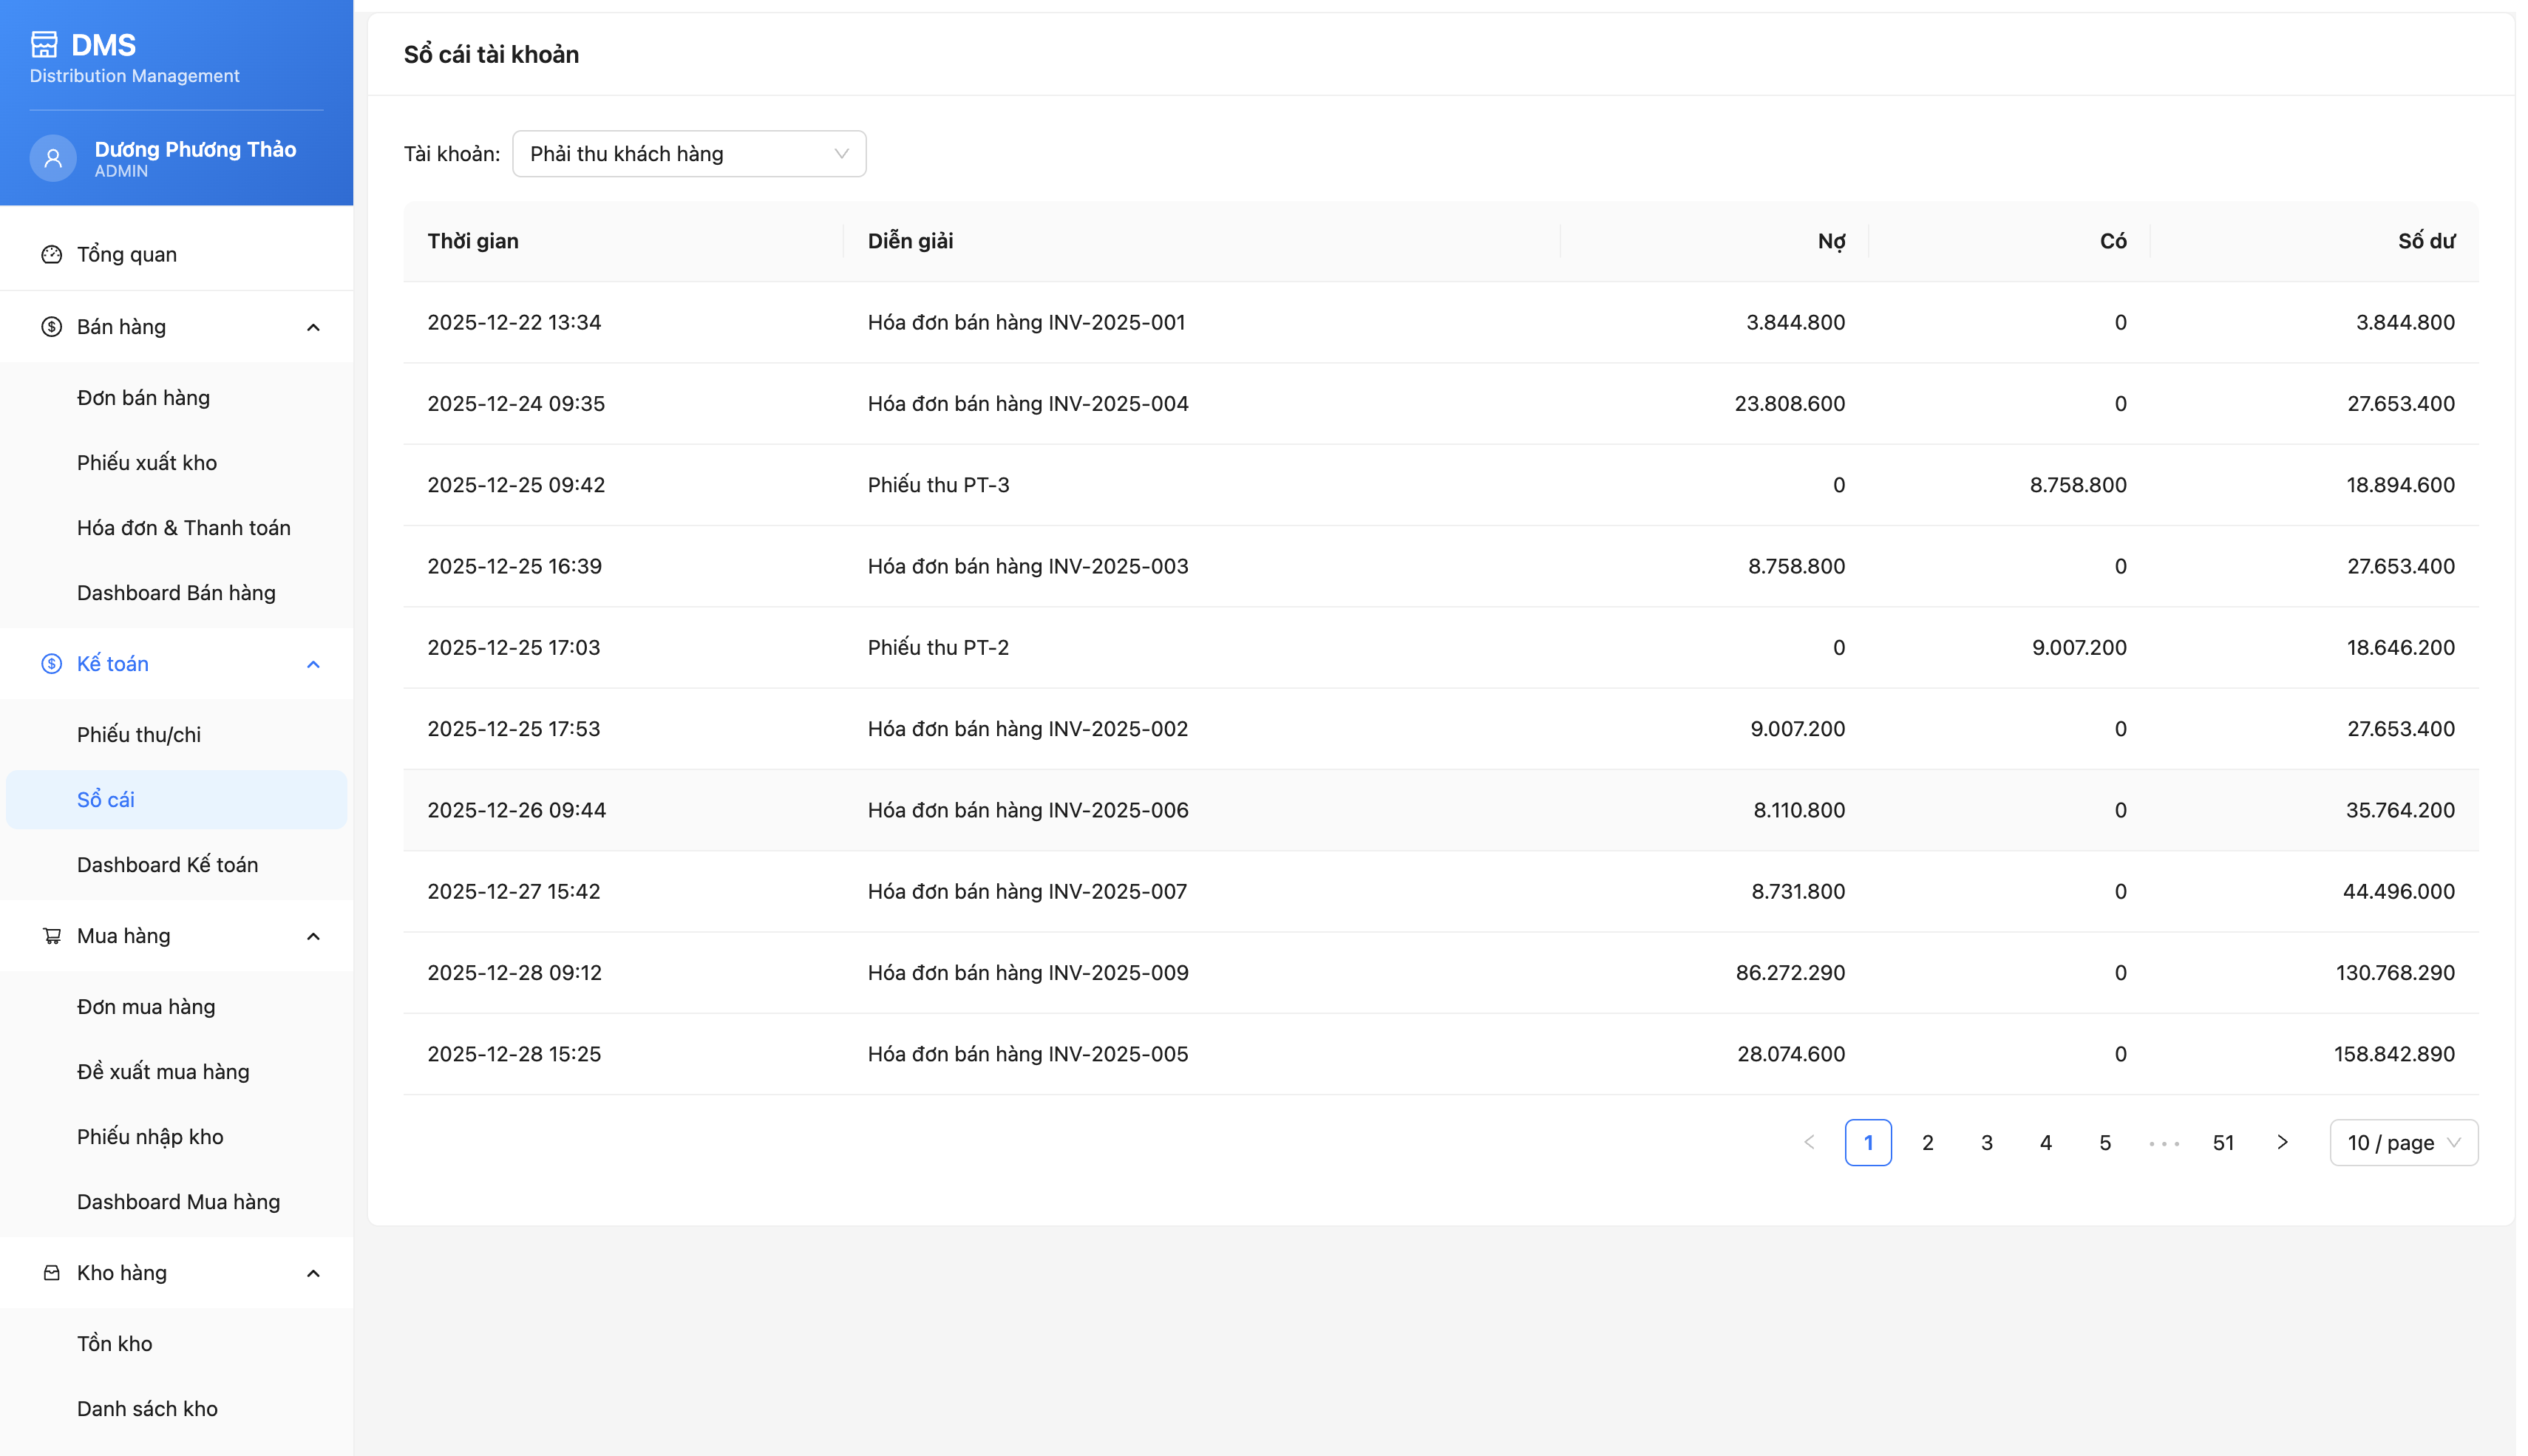
\includegraphics[width=0.95\linewidth]{Figure/screenshots/10-payment-ledger.png}
\caption{Accounts-receivable ledger with running balance}\label{fig:ui-ledger}
\end{figure}

Figure~\ref{fig:ui-ledger} shows the ledger of the accounts-receivable account.
Every sales invoice posts a debit entry and every payment receipt posts a credit
entry, and the running-balance column on the right is recomputed after each
posting. Because the same posting that debits this account credits the
corresponding revenue or cash account, the ledger is the user-facing evidence of
the double-entry accounting model described in Chapter~\ref{chapter:Contribution}.

Taken together, these screenshots confirm that the implemented system realises the
full inbound-to-settlement workflow on real data. The next section reports how the
business rules underlying these functions are verified by automated and manual
tests.

\section{Testing}
The system was verified with two complementary techniques: automated tests that
pin down the business rules with the highest consistency risk, and manual
end-to-end scenario tests that exercise the full workflow through the user
interface.

\subsection{Automated tests}
The automated suite contains thirteen tests grouped into seven classes. It runs
on an in-memory H2 database under the \texttt{test} Spring profile, so it is
self-contained and repeatable without an external database. Table~\ref{tab:autotests}
summarises the suite; all thirteen tests pass. The tests deliberately target the
points where correctness is hardest to guarantee: first-expired-first-out (FEFO)
lot allocation, stock reservation, concurrent stock deduction, double-entry
ledger balances, the credit-limit rule, and endpoint authorisation.

\begin{table}[H]\centering
\caption{Automated test suite (all passing)}
\label{tab:autotests}
\resizebox{\linewidth}{!}{%
\begin{tabular}{|l|c|l|}
\hline
\textbf{Test class} & \textbf{Tests} & \textbf{Verifies} \\ \hline
FefoAllocationTest & 2 & FEFO query order; earliest-expiry lot consumed first \\ \hline
ReservationTest & 3 & reserve raises reserved and lowers available; over-reserve rejected \\ \hline
ConcurrencyLotTest & 1 & two concurrent issues serialised; no lost update at lot level \\ \hline
AccountingServiceTest & 2 & running ledger balance; zero-amount postings skipped \\ \hline
CreditLimitRuleTest & 3 & credit-limit rule evaluated at the boundary \\ \hline
RbacSecurityTest & 1 & protected endpoint without a token is rejected \\ \hline
CoreFlowTest & 1 & application context loads with all beans wired \\ \hline
\end{tabular}%
}
\end{table}

\subsection{Critical-function test cases}
Table~\ref{tab:tests} lists the three most important functional cases together
with their observed results. TC01 is the most important case because it checks
both the aggregate inventory and the lot-level FEFO deduction: with two lots of
different expiry dates, the earliest-expiry lot is fully consumed before any
quantity is taken from the later lot. TC02 checks that reserving stock raises the
reserved quantity and lowers the available quantity while the on-hand quantity is
unchanged, which prevents overselling before goods leave the warehouse. TC03
checks the credit-limit rule, which rejects a purchase when the resulting balance
would exceed the customer credit limit.

\begin{table}[H]\centering
\caption{Critical-function test cases and results}
\label{tab:tests}
\resizebox{\linewidth}{!}{%
\begin{tabular}{|c|l|l|l|c|}
\hline
\textbf{ID} & \textbf{Function} & \textbf{Input} & \textbf{Expected} & \textbf{Result} \\ \hline
TC01 & Confirm GI (FEFO) & two lots, near/far expiry & earliest-expiry lot consumed first & Pass \\ \hline
TC02 & Approve SO (reserve) & qty $\leq$ available & reserved up, available down, on-hand same & Pass \\ \hline
TC03 & Credit-limit rule & balance+amt $>$ limit & purchase rejected by the rule & Pass \\ \hline
\end{tabular}%
}
\end{table}

The three cases are backed by \texttt{FefoAllocationTest}, \texttt{ReservationTest},
and \texttt{CreditLimitRuleTest} respectively, so they are reproducible rather than
one-off manual checks. One limitation is recorded for transparency: the
credit-limit rule is implemented and tested as a domain method, but it is not yet
invoked in the sales-order approval path, which currently enforces only stock
availability; connecting the rule to order approval is left as future work. In
addition to the automated suite, the full business workflow PO $\to$ GR $\to$ SO
approval $\to$ GI $\to$ delivery $\to$ invoice $\to$ payment was exercised
manually through the web interface against a seeded database, and the resulting
screens are presented earlier in this chapter as the illustration of the main
functions.

\section{Deployment}
\label{sec:deployment}
% GUIDE: deployment model, server/equipment specs, configuration, and any test
% deployment results (users, response time, load).
\thesisfig{deployment}{Deployment diagram}{fig:deploy}
The deployment model in Figure~\ref{fig:deploy} contains three runtime
components. The React frontend is served by the Vite development server during
development at port 5173, or by a static web server in a production-like
deployment. The Spring Boot backend runs as a Java application at port 8080 and
exposes REST APIs under \texttt{/api}. PostgreSQL runs as the database server,
using the default port 5432 in the local development environment.

For local demonstration, the backend is started with \texttt{mvn
spring-boot:run} and the frontend is started with \texttt{npm run dev}. The
frontend communicates with the backend through Axios. Authentication requests
return JWT tokens, and subsequent API calls include the token for authorization.
The backend connects to PostgreSQL using the configuration in
\texttt{application.yml}. In a production deployment, the same logical structure
can be placed behind a reverse proxy, with HTTPS termination at the proxy and
environment variables used for database credentials and JWT secrets.


\newpage
\chapter{SOLUTION AND CONTRIBUTION}
\label{chapter:Contribution}
% ===================== CHAPTER 5 — SOLUTION AND CONTRIBUTION =====================
% Length: >= 5 pages. THE chapter graders weight most. Present each contribution in a
% section with: (i) problem, (ii) solution, (iii) results. Do NOT repeat earlier detail
% verbatim — earlier chapters should cross-reference here.
This chapter presents the principal contributions of the thesis. Each contribution
is described through the problem it addresses, the proposed solution, and the
results achieved.

\section{FEFO Lot-Allocation Mechanism}
% (i) Problem: perishable goods must leave by earliest expiry to reduce waste, while
%     keeping a per-lot audit trail. A plain quantity-only stock model cannot do this.
% (ii) Solution: an InventoryLot model + a FEFO query (ORDER BY expiryDate ASC NULLS
%     LAST) that greedily consumes the earliest-expiring lots on goods issue, recording
%     the batch/expiry on each issue line. (Reference: GoodsIssueServiceImpl.)
% (iii) Results: oldest stock exits first; full traceability; expiry alerts.
\thesisfig{flowchart_fefo}{FEFO allocation algorithm}{fig:fefo}
The first contribution is the lot-allocation mechanism for perishable goods.
For date-sensitive stock, inventory theory recommends issuing the
earliest-expiring units first so that shrinkage from expiry is
minimised~\cite{silver1998inventory, richards2021warehouse}. Commercial
distribution systems therefore provide batch and expiry tracking, for example the
lot and removal-strategy features of Odoo~\cite{odooFefo} and the batch
management of SAP Business One~\cite{sapBatch}. Many lighter-weight systems,
however, keep only an aggregate quantity for each product and warehouse. This
model is sufficient for simple stock checking, but it cannot answer which batch
should be picked first, which expiry date was delivered to a customer, or which
remaining lots are close to expiry. For a distributor that handles food,
medicine, cosmetics, or other date-sensitive goods, this limitation directly
creates waste and traceability risk.

The proposed solution extends the aggregate inventory model with an
\texttt{InventoryLot} entity. Each lot stores the product, warehouse, lot number,
expiry date, quantity received, quantity remaining, unit cost, and the source
goods receipt item. When a goods receipt is confirmed, the accepted quantity
increases aggregate inventory and also creates a corresponding inventory lot.
The implementation prevents duplicate lot creation for the same receipt item by
checking whether a source receipt item has already generated a lot. This keeps
goods receipt confirmation safe when the operation is retried after an
interrupted request.

During goods issue confirmation, the service retrieves all available lots for
the product and warehouse ordered by FEFO: lots with an expiry date come first,
the earliest expiry date is selected before later ones, and lots without expiry
dates are placed last. The service validates that the sum of remaining lot
quantity can cover the requested issue quantity. It then greedily consumes lots
in this order until the requested quantity is fully allocated. The first consumed
lot number and expiry date are copied to the goods issue item so that the
outbound document displays the batch information used for picking.

\begin{algorithm}[H]
\caption{FEFO allocation for a goods-issue item}
\KwIn{product, warehouse, issueQuantity}
\KwOut{updated lots and goods-issue line batch information}
lots $\leftarrow$ find available lots ordered by expiry date ascending\;
\If{sum(lot.quantityRemaining) $<$ issueQuantity}{
  reject confirmation with an insufficient-lot-stock error\;
}
remaining $\leftarrow$ issueQuantity\;
\ForEach{lot in lots}{
  \If{remaining = 0}{break}
  take $\leftarrow$ min(remaining, lot.quantityRemaining)\;
  lot.quantityRemaining $\leftarrow$ lot.quantityRemaining - take\;
  remaining $\leftarrow$ remaining - take\;
}
record the first consumed lot number and expiry date on the goods-issue item\;
\end{algorithm}

The achieved result is a practical FEFO process integrated with the order and
warehouse workflow. The system no longer relies on the warehouse employee to
manually choose a batch after reading several spreadsheets. Earlier-expiring
stock is consumed first, remaining lot quantities are visible for expiry
monitoring, and outbound documents keep the batch information needed for later
traceability.

% You may also typeset the algorithm with algorithm2e, e.g.:
% \begin{algorithm}[H]\caption{FEFO allocation}\dots\end{algorithm}

\section{Concurrency Control for Lot-Level Stock Deduction}
% (i) Problem: the FEFO lot deduction is a read-modify-write on InventoryLot, which has
%     no version/row lock. Two simultaneous goods-issue confirmations on the same scarce
%     product can both pass validation and both deduct -> lost update at lot level; the
%     per-lot ledger over-draws and diverges from the aggregate.
% (ii) Solution: acquire a pessimistic write lock (SELECT ... FOR UPDATE) on the single
%      aggregate Inventory row at the start of confirm(), before any lot is read, ordered
%      by ascending productId to prevent deadlock. (lockInventoryForUpdate.)
% (iii) Results: the conflicting confirmations are serialized at the database; the lot
%       ledger stays consistent with the aggregate.
The next contribution hardens the goods-issue path against a concurrency
hazard in the lot deduction described earlier in this chapter. The FEFO
allocation is a read-modify-write sequence: the service reads the remaining
quantity of each lot, computes how much to take, and writes the reduced
quantity back. The aggregate \texttt{Inventory} row is already protected, both
by an optimistic version field and by a pessimistic read in
\texttt{decreaseInventory} that issues a \texttt{SELECT~\dots~FOR~UPDATE}. The
per-lot \texttt{InventoryLot} entity, however, carries neither a version column
nor a row lock. When two warehouse staff confirm goods issues for the same
scarce product at almost the same time, both transactions can read the same lot
quantities, both can pass the validation that the remaining lot quantity covers
the requested amount, and both can deduct from the same lots. The second write
silently overwrites the first, which is the classic lost-update anomaly. The
result is a per-lot ledger that over-draws a lot or drives its remaining
quantity negative, so the sum of lot quantities no longer reconciles with the
aggregate on-hand quantity, defeating the traceability the lot model was built
to provide.

The proposed solution serializes the entire deduction of a product behind the
aggregate inventory row, which is the only record shared by every goods issue
for that product and warehouse. At the very start of the confirmation, before
any lot is read, the service acquires a pessimistic write lock on each
relevant \texttt{Inventory} row through a dedicated
\texttt{lockInventoryForUpdate} operation. This operation reuses the existing
\texttt{SELECT~\dots~FOR~UPDATE} query but does not modify the row; its only
purpose is to claim the lock. Because the lock is taken inside the
confirmation's transaction, the database holds it until that transaction
commits or rolls back~\cite{postgresql14}. A competing confirmation for the
same product therefore blocks on this single row, and when it finally proceeds
it re-reads the lots with the already-updated quantities rather than the stale
ones. In effect, the aggregate row acts as a gate that protects not only the
aggregate deduction but the unguarded lot read-modify-write as well. This is an
application of the pessimistic offline lock pattern, in which a shared record is
locked for the whole duration of a business transaction to prevent concurrent
modification~\cite{fowler2002poeaa, bauer2015hibernate}.

A goods issue may contain several products, so a single confirmation can lock
several inventory rows. To avoid a deadlock in which one transaction holds the
lock on product A while waiting for product B and a second transaction holds B
while waiting for A, the service collects the distinct product identifiers and
acquires the locks in ascending identifier order. Because every confirmation
takes the locks in the same global order, a cycle of mutual waiting cannot
form, which is the standard ordered-locking discipline for deadlock
prevention~\cite{fowler2002poeaa}.

The result is that two conflicting goods-issue confirmations for the same
product no longer interleave; the second is queued at the database until the
first completes, after which it observes a consistent state. The lot ledger
stays reconciled with the aggregate on-hand quantity even under concurrent
issue, which closes the lost-update gap while keeping the database schema
unchanged, since the fix reuses the existing aggregate row rather than adding a
version column to every lot. The accepted trade-off is reduced parallelism for
issues that touch the same product; this is acceptable because such operations
are inherently conflicting and must be ordered for correctness. This behaviour
is guarded by a deterministic two-thread integration test
(\texttt{ConcurrencyLotTest}) in which both confirmations are released
simultaneously through a shared barrier: with the lock in place exactly one
issue succeeds and the lot ledger stays consistent with the aggregate on-hand
quantity, whereas removing the lock reintroduces the lost update.

\section{Inventory Reservation on Order Approval}
% (i) Problem: overselling between approval and shipment.
% (ii) Solution: reserve stock at SO approval (quantityReserved up, quantityAvailable
%      down); deduct only at goods-issue confirmation; release on cancel.
% (iii) Results: no oversell; clear available-vs-reserved visibility.
The second contribution is inventory reservation at the moment a sales order is
approved. In a manual process, two sales staff members may check the same
physical stock and both promise it to different customers. Even if the stock is
physically sufficient at the first check, the company can oversell before the
warehouse confirms goods issue. This problem appears in the interval between
sales approval and physical shipment, and it corresponds to the
available-to-promise concept in supply chain planning, where committed stock must
be separated from free stock before an order is confirmed~\cite{chopra2019supply}.

The system addresses this issue by separating on-hand, reserved, and available
quantities. When a sales order is approved, the service checks available
quantity for each order line in the selected warehouse. If every line can be
fulfilled, it increases the reserved quantity and reduces the available quantity.
The physical on-hand quantity is not reduced at this stage because the goods are
still in the warehouse. When the goods issue is later confirmed, the system
deducts on-hand quantity and releases the corresponding reservation. If an
approved order is cancelled before shipment, only the remaining reserved
quantity is released.

This design gives different business users the right view of stock. Sales staff
see available quantity, which prevents them from selling stock that is already
committed. Warehouse staff still see the physical on-hand quantity for picking
and reconciliation. Managers can distinguish between real stock shortage and
stock that is present but reserved for approved orders. As a result, the system
reduces overselling risk without prematurely deducting stock before goods leave
the warehouse.

\section{Failed-Delivery Recovery}
% (i) Problem: a failed delivery must cleanly reverse stock, invoice and order state.
% (ii) Solution: restockFromFailedDelivery() restores inventory + lots, cancels the
%      invoice (warns if already paid), resets delivered qty, reverts SO status.
% (iii) Results: consistent, idempotent recovery.
The third contribution is a centralized recovery mechanism for failed delivery.
In the order-to-cash workflow, a confirmed goods issue has already deducted
stock, updated delivered quantities, and generated an invoice. If the delivery
later fails, a manual correction must reverse several records in the right order.
If only one record is corrected, the system becomes inconsistent: inventory may
show fewer goods than the warehouse has, the order may appear delivered, or the
invoice may remain active although the customer did not receive the goods.

The system implements this recovery in \texttt{restockFromFailedDelivery}. The
method finds the goods issue linked to the failed trip, adds the issued quantity
back to aggregate inventory, restores the quantity to the corresponding lot,
decreases the delivered quantity of the sales order item, cancels the invoice
when it is still cancellable and unpaid, and recalculates the sales order
delivery status. If the invoice already has payment, the system does not
silently cancel it; instead it records a warning so that the accountant can
perform refund or adjustment work manually. This is important because financial
documents should not be reversed automatically after money has been collected.

The result is that delivery failure is treated as a business event rather than a
set of unrelated manual edits. The recovery path protects the consistency among
inventory, lots, sales orders, and invoices. In the current implementation, the
method is intended to be called from a controlled delivery-status transition; a
future improvement is to add an explicit recovery marker on the goods issue or
delivery order to make repeated calls harmless at the database level.

\section{Role-Based Workflow Enforcement}
% (i) Problem: separation of duties (creator != approver) across 9 roles.
% (ii) Solution: RBAC at endpoint + method + data level (e.g. shippers see only their
%      own trips via isAssignedTo()).
% (iii) Results: enforced approval chains and least-privilege access.
The fourth contribution is role-based workflow enforcement. The distribution
process involves several responsibilities: staff create documents, managers or
accountants approve them, warehouse staff confirm physical stock movements,
delivery administrators assign trips, and shippers update only their assigned
deliveries. If all users could access all operations, the system would lose
separation of duties and approval would become only a visual status rather than
a real control. This requirement is an instance of the role-based access control
model, in which permissions are assigned to roles rather than to individual
users, and which supports separation of duties and least
privilege~\cite{sandhu2000nist}.

The system defines nine roles and applies access control at three levels. At the
endpoint level, Spring Security restricts URL patterns and HTTP methods, for
example allowing only purchase managers, accountants, or administrators to
approve purchase orders. At the method level, \texttt{@PreAuthorize} annotations on individual
controller endpoints restrict sensitive operations, such as approving and
rejecting orders, recording payments, and managing user accounts, to the roles
permitted to perform them. At the data level, services enforce contextual
constraints, such as preventing warehouse staff from seeing unapproved orders
and limiting shippers to assigned trips. Table~\ref{tab:rbac-matrix} summarises
the main permission groups.

\begin{table}[H]\centering
\caption{Simplified RBAC permission matrix}
\label{tab:rbac-matrix}
\small
\resizebox{\linewidth}{!}{%
\begin{tabular}{|p{3.6cm}|c|c|c|c|c|c|}
\hline
\textbf{Role} & \textbf{PO} & \textbf{SO} & \textbf{GR/GI} & \textbf{Delivery} & \textbf{Invoice} & \textbf{Users} \\ \hline
Administrator & Full & Full & Full & Full & Full & Full \\ \hline
Purchase staff & Create/Edit & View & View GR & No & No & No \\ \hline
Purchase manager & Approve & View & View GR & No & No & No \\ \hline
Sales staff & View & Create/Edit & View GI & No & View & No \\ \hline
Sales manager & View & Approve & View GI & No & Manage & No \\ \hline
Warehouse staff & Approved only & Approved only & Confirm & No & No & No \\ \hline
Delivery administrator & No & View & View & Manage & No & No \\ \hline
Shipper & No & No & No & Assigned trips & No & No \\ \hline
Accountant & Approve & Approve & View & No & Manage & No \\ \hline
\end{tabular}%
}
\end{table}

This design makes the workflow enforceable by the application instead of relying
only on organizational discipline. It also improves usability because each user
sees a smaller set of relevant actions. The result is a least-privilege
prototype that supports approval chains, warehouse control, delivery assignment,
and financial visibility while keeping administrative functions restricted.

\section{Eliminating N+1 Queries in Delivery Listing}
% (i) Problem: object-relational N+1 — one extra query per row + lazy loads made the
%     available-delivery-order listing scale linearly with data and become slow.
% (ii) Solution: replace per-row queries with three bulk queries (orders mapped by code,
%     planned order ids as a set, confirmed goods issues with fetch-joined associations).
% (iii) Results: endpoint latency 2380 ms -> 47 ms on the same dataset (~50x).
The fifth contribution is a performance optimisation of the screen that lists the
delivery orders available for planning. This endpoint is opened frequently by the
delivery administrator, so its responsiveness affects daily operation directly.
The original implementation iterated over every confirmed goods issue and, for
each one, executed a separate query to look up the matching delivery order by
code and another query to check whether that order already belonged to a delivery
plan. Because the sales order, customer, and delivery address of each goods issue
were mapped lazily, accessing them inside the loop triggered further queries. This
is the well-known object-relational \emph{N+1 select} problem documented in the
object-relational mapping literature~\cite{bauer2015hibernate}: the number of
database round trips grows linearly with the number of rows, so the response time
degrades as the data set grows. On the development data set the listing endpoint
took approximately 2380~ms.

The optimisation replaces the per-row queries with three bulk queries executed
once before the loop. The first loads every delivery order and indexes it by code
in an in-memory map, so the matching order is resolved by a hash lookup instead of
a database query. The second loads the identifiers of all delivery orders that
already belong to a plan as a single projection and stores them in a set, so the
``already planned'' test becomes a set membership check. The third loads the
confirmed goods issues with their sales order, customer, and delivery address
eagerly through a \texttt{JOIN FETCH} query, which removes the lazy-loading round
trips inside the loop. The loop then only creates a delivery order in the rare
case that one has not yet been materialised for a newly confirmed goods issue.

The result is a substantial latency reduction: on the same data set and
environment the endpoint response time fell from approximately 2380~ms to
47~ms, an improvement of roughly fifty times, while the returned data is
unchanged. The number of database round trips no longer depends on the number of
goods issues, so the listing remains responsive as the volume of confirmed
shipments grows. This contribution demonstrates that the system was not only
built to be functionally correct but was also profiled and tuned at the data
access layer, which is a common source of performance problems in applications
built on an object-relational mapping framework such as Spring Data JPA and
Hibernate~\cite{springboot314}.


\newpage
\chapter{CONCLUSION AND FUTURE WORK}
\label{chapter:Conclusion}
% ===================== CHAPTER 6 — CONCLUSION AND FUTURE WORK =====================
\section{Conclusion}
% GUIDE: compare results with similar products; state what was/was not achieved;
% identify the main contributions; note lessons learned.
This thesis has designed and implemented a web-based supply-chain management
system for small and medium-sized distributors. Compared with broad ERP products
such as Odoo and SAP Business One, the system is narrower in scope but more
focused on the workflow selected for the thesis: purchase approval, goods
receipt, lot-based inventory, sales order approval, stock reservation, FEFO
goods issue, delivery execution, invoice generation, dashboard reporting, and
role-based access control. Compared with retail-oriented systems such as
KiotViet, Sapo, and MISA, the prototype emphasizes distributor workflow
integration rather than point-of-sale operation.

The main achieved result is a working application structure that connects the
procure-to-stock and order-to-cash processes. In terms of scale, the
requirements were modelled as nine actors and seven fully specified use cases
(Chapter~\ref{chapter:Survey}) realised over a relational schema of thirty-two
tables; the backend contains 176 Java classes with 11,821 lines of source code
and the frontend 10,575 lines of JavaScript/JSX, both measured with the
\texttt{cloc} tool excluding blank and comment lines, and the business rules
with the highest consistency risk are pinned by fifteen automated tests. The
system implements the core modules required by the project scope: master data,
purchasing, goods receipt, inventory, lot management, sales, goods issue,
invoice, accounting, customer payment, delivery, dashboard, authentication, and
user management. Measured on a realistic dataset of approximately eight thousand
transactional rows, the principal read endpoints respond in under sixty
milliseconds on average, and a targeted optimisation of the delivery-listing
endpoint reduced its response time from about 2{,}380~ms to 47~ms
(Section~\ref{sec:perf}).

The key contributions are the FEFO lot-allocation mechanism, the inventory
reservation mechanism at sales order approval, the failed-delivery recovery
procedure, and the role-based workflow enforcement. These contributions address
the most important risks of a distributor: expired stock, overselling,
inconsistent recovery after delivery failure, and uncontrolled access to
approval and warehouse operations.

Several limitations remain, and stating them precisely is more useful than
overstating the result. The system is a prototype validated in a
single-organisation, single-instance setting. Its performance was measured only
under sequential requests against one backend instance
(Section~\ref{sec:perf}); behaviour under high concurrent load has not been
load-tested, and the system has not been evaluated through long-term operation
in a real production environment. On the functional side, although the
accounting module records simplified double-entry journal entries (each with a
debit and a credit account) automatically from source documents and tracks
customer payments, it does not yet produce full financial statements such as
balance sheets and income statements, perform period-end closing, or integrate
with external accounting software, and the system does not yet support automatic
route optimisation, barcode scanning, or demand forecasting.

\section{Future Work}
% GUIDE: first, work needed to complete existing features; then new directions
% (e.g. route optimisation for delivery, demand forecasting, barcode/QR scanning,
% mobile shipper app, multi-warehouse transfer, reporting/BI).
Future work should first complete and harden the existing functions. Although the
rules with the highest consistency risk are already covered by automated tests
(Chapter~\ref{chapter:Design}), the test set should be extended to the flows that
are currently exercised only through manual end-to-end scenarios, namely
goods-receipt confirmation, sales-order cancellation, and failed-delivery
recovery. The failed-delivery mechanism should add an explicit
database-level recovery marker so that repeated calls cannot restore the same
goods issue twice. The performance evaluation should also be extended from
sequential measurement to a concurrent load test that establishes the
throughput and tail latency the system sustains as the number of simultaneous
users grows. The reporting module should be validated with larger sample data.

At the architectural level, the goods-issue path currently serialises concurrent
deductions with pessimistic write locks taken on the affected \texttt{Inventory}
rows, acquired in ascending product-identifier order to prevent deadlock
(Chapter~\ref{chapter:Design}). This guarantees that lot quantities cannot be
lost-updated, but it also turns those rows into a serialisation point that could
become a throughput bottleneck if transaction volume rises sharply. A natural
evolution is to move toward an event-driven architecture in which stock-issue
requests are placed on a message broker such as Apache Kafka or RabbitMQ and
consumed asynchronously \cite{hohpe2003eip, kleppmann2017ddia}. Processing the
issue commands through a queue would relieve the direct lock contention on the
relational database and decouple request acceptance from stock settlement, at
the cost of an eventual-consistency model that the user interface and the
reservation logic would have to accommodate.

The next development direction is to improve warehouse and delivery efficiency.
Barcode or QR scanning can reduce manual input errors during goods receipt,
goods issue, and inventory counting. A mobile-friendly shipper interface or
dedicated mobile application can make delivery updates easier outside the
office. Route optimization can help delivery administrators reduce travel time
and fuel cost when assigning orders to trips. Multi-warehouse transfer should be
added for distributors that move stock between warehouses before shipment.

Another direction is decision support. Demand forecasting can use historical
sales data to suggest reorder quantities. Business intelligence dashboards can
provide deeper analysis of revenue, stock turnover, expired stock, customer
debt, and supplier performance. Finally, the accounting module can be extended
with financial statements, period-end closing, payment reconciliation, and
integration with external accounting software.

A further refinement concerns the integrity of accounting records during
failed-delivery recovery. At present the system cancels the sales invoice
attached to a failed delivery only while that invoice is still in a cancellable
state and no payment has been recorded against it; once a payment exists,
cancellation is withheld and the case is escalated for manual settlement
(Chapter~\ref{chapter:Design}). A more rigorous approach, consistent with
accounting practice, is to treat an issued document as immutable and never
delete it: rather than cancelling the invoice, the system would automatically
generate a credit note that offsets the customer's receivable. This would
preserve a complete audit trail for every issued document, unify the paid and
unpaid cases under a single rule, and align the recovery procedure with the
controls expected of an accounting information system \cite{romney2021ais}.


% ===================================================
\newpage
\renewcommand\bibname{REFERENCE}
\printbibliography
\phantomsection\addcontentsline{toc}{chapter}{REFERENCE}

\appendixpage
\appendices
\addappheadtotoc
\renewcommand{\figurename}{Figure}
\renewcommand{\tablename}{Table}
\renewcommand{\chaptername}{CHAPTER}

\titleformat{\chapter}[hang]{\centering\bfseries}{ \thechapter.\ }{0pt}{}[]
\titlespacing*{\chapter}{0pt}{-20pt}{20pt}
\titlecontents{chapter}[0.0cm]{\bfseries\vspace{0.3cm}}{{\bfseries{\scshape} \thecontentslabel.\ }}{}{\titlerule*[0.3pc]{.}\contentspage}

\chapter{ADDITIONAL USE CASE DESCRIPTIONS}
% ===================== APPENDIX — ADDITIONAL USE CASE DESCRIPTIONS =====================
% GUIDE: detailed specs for use cases that did not fit in Chapter 2 (same format:
% name, event flow main+alternate, pre-conditions, post-conditions).

\section*{Use case: Record Customer Payment}
[TODO] Specify the use case.

\section*{Use case: Adjust Stock}
[TODO] Specify the use case.

\section*{Use case: Monitor Expiring Lots}
[TODO] Specify the use case.

\end{document}
